% ============================================================
%  RAPPORT DE STAGE — Systeme RAG (Retrieval-Augmented Generation)
%  Stage Data Science — Ete 2026
%
%  Compilation :  pdflatex main  ->  pdflatex main   (2 passes)
%             ou :  make
%             ou :  deposer le dossier sur Overleaf
% ============================================================
\documentclass[12pt,a4paper,oneside]{report}

% ------------------------------------------------------------
%  >>> INFORMATIONS A VERIFIER / ADAPTER <<<
%  Ces valeurs alimentent la page de garde et les metadonnees PDF.
% ------------------------------------------------------------
\newcommand{\reporttitle}{Construction d'un Système RAG pour l'Automatisation de la Recherche d'Information en Entreprise}
\newcommand{\reportsubtitle}{Assistant documentaire interne à réponses sourcées}
\newcommand{\authorname}{TLILI Mohamed Aziz}
\newcommand{\supervisor}{Mme ENNINE Hanene}
\newcommand{\organism}{ESPRIT-Tech}
\newcommand{\academicyear}{2025 / 2026}
\newcommand{\speciality}{DATA SCIENCE}
\newcommand{\internshipduration}{2 mois}

% ============================================================
%  Préambule — packages, mise en page, styles
% ============================================================

% --- Encodage & langue ---------------------------------------
\usepackage[utf8]{inputenc}
\usepackage[T1]{fontenc}
\usepackage[french]{babel}
\usepackage{lmodern}
\usepackage{textcomp}

% --- Mise en page --------------------------------------------
\usepackage[a4paper,left=2.5cm,right=2.5cm,top=2.5cm,bottom=2.5cm]{geometry}
\usepackage{setspace}
\onehalfspacing
\usepackage{parskip}
\setlength{\parindent}{1em}

% --- Graphiques & couleurs -----------------------------------
\usepackage{graphicx}
\graphicspath{{images/}}
\usepackage{xcolor}
\usepackage{tikz}
\usetikzlibrary{shapes.geometric,arrows.meta,positioning,calc,fit,backgrounds}

% --- Tableaux -------------------------------------------------
\usepackage{booktabs}
\usepackage{tabularx}
\usepackage{longtable}
\usepackage{multirow}
\usepackage{array}
\renewcommand{\arraystretch}{1.25}

% --- Maths ----------------------------------------------------
\usepackage{amsmath}
\usepackage{amssymb}

% --- Listes ---------------------------------------------------
\usepackage{enumitem}
\setlist{itemsep=2pt,parsep=0pt,topsep=4pt}

% --- Légendes -------------------------------------------------
\usepackage{caption}
\captionsetup{font=small,labelfont=bf,labelsep=endash}

% --- Palette --------------------------------------------------
\definecolor{accent}{HTML}{0E7C7B}
\definecolor{ink}{HTML}{1C2B39}
\definecolor{muted}{HTML}{5B6660}
\definecolor{soft}{HTML}{EEF1EF}
\definecolor{warn}{HTML}{C77D2E}
\definecolor{codebg}{HTML}{F7F8F7}
\definecolor{codekw}{HTML}{0B5FA5}
\definecolor{codestr}{HTML}{9C5A20}
\definecolor{codecom}{HTML}{6A7370}

% --- Code source ----------------------------------------------
\usepackage{listings}
\lstset{
  basicstyle=\ttfamily\footnotesize,
  keywordstyle=\color{codekw}\bfseries,
  stringstyle=\color{codestr},
  commentstyle=\color{codecom}\itshape,
  backgroundcolor=\color{codebg},
  frame=leftline,
  framesep=6pt,
  rulecolor=\color{accent},
  framerule=1.6pt,
  numbers=none,
  breaklines=true,
  breakatwhitespace=true,
  showstringspaces=false,
  columns=fullflexible,
  keepspaces=true,
  xleftmargin=10pt,
  aboveskip=10pt,
  belowskip=10pt,
  extendedchars=true,
  literate=%
    {é}{{\'e}}1 {è}{{\`e}}1 {ê}{{\^e}}1 {ë}{{\"e}}1
    {à}{{\`a}}1 {â}{{\^a}}1 {ä}{{\"a}}1
    {ù}{{\`u}}1 {û}{{\^u}}1 {ü}{{\"u}}1
    {î}{{\^i}}1 {ï}{{\"i}}1
    {ô}{{\^o}}1 {ö}{{\"o}}1
    {ç}{{\c c}}1
    {É}{{\'E}}1 {È}{{\`E}}1 {Ê}{{\^E}}1
    {À}{{\`A}}1 {Ç}{{\c C}}1
    {«}{{\guillemotleft}}1 {»}{{\guillemotright}}1
    {’}{{'}}1 {—}{{---}}1 {–}{{--}}1
}
\lstdefinestyle{python}{language=Python}
\lstdefinestyle{bash}{language=bash}
\lstdefinestyle{plain}{language=}

% --- En-têtes & pieds de page --------------------------------
\usepackage{fancyhdr}
\pagestyle{fancy}
\fancyhf{}
\fancyhead[L]{\small\nouppercase{\leftmark}}
\fancyhead[R]{\small\nouppercase{\rightmark}}
\fancyfoot[C]{\thepage}
\renewcommand{\headrulewidth}{0.4pt}
\renewcommand{\footrulewidth}{0pt}

\fancypagestyle{plain}{%
  \fancyhf{}%
  \fancyfoot[C]{\thepage}%
  \renewcommand{\headrulewidth}{0pt}%
}

\renewcommand{\chaptermark}[1]{\markboth{\chaptername~\thechapter.\ #1}{}}
\renewcommand{\sectionmark}[1]{\markright{\thesection.\ #1}}

% --- Titres de chapitre ---------------------------------------
\usepackage{titlesec}
\titleformat{\chapter}[display]
  {\normalfont\huge\bfseries\color{ink}}
  {\normalfont\normalsize\color{accent}\MakeUppercase{\chaptertitlename}\ \Huge\thechapter}
  {12pt}{\Huge}
\titlespacing*{\chapter}{0pt}{10pt}{28pt}

% --- Liens ----------------------------------------------------
% URL longues : autoriser la coupure aux separateurs pour qu'elles
% ne debordent pas de la marge dans la bibliographie.
\usepackage[hyphens]{url}
\Urlmuskip=0mu plus 1mu\relax
\def\UrlBreaks{\do\/\do\-\do\.\do\_\do\?\do\&\do\=\do\+\do\:}

\usepackage[hidelinks,breaklinks=true,plainpages=false]{hyperref}
\hypersetup{
  colorlinks=true,
  linkcolor=ink,
  citecolor=accent,
  urlcolor=accent,
  pdftitle={Rapport de stage - Systeme RAG},
  pdfauthor={\authorname}
}

% ============================================================
%  Commandes utilitaires
% ============================================================

% Valeur à compléter après exécution de l'évaluation RAGAS.
% Rend le trou visible à la relecture : remplacer par le chiffre mesuré.
\newcommand{\aremplir}[1]{\textcolor{warn}{\textbf{#1}}}

% Terme technique en anglais
\newcommand{\eng}[1]{\emph{#1}}

% Encadré "note"
\usepackage{mdframed}
\newmdenv[
  linecolor=accent,
  linewidth=1.6pt,
  topline=false,bottomline=false,rightline=false,
  backgroundcolor=soft,
  innerleftmargin=10pt,innerrightmargin=10pt,
  innertopmargin=8pt,innerbottommargin=8pt,
  skipabove=10pt,skipbelow=10pt
]{encadre}


\begin{document}

% ============================================================
%  PARTIE LIMINAIRE  (numerotation romaine)
% ============================================================
\pagenumbering{roman}

% ============================================================
%  Page de garde
%  On evite l'environnement `titlepage` : il remet le compteur de
%  page a 1, ce qui cree deux pages numerotees "i" et provoque des
%  destinations PDF dupliquees.
% ============================================================
\thispagestyle{empty}
\begingroup
\centering

\vspace*{0.6cm}

{\large\scshape République Tunisienne\par}
{\large\scshape Ministère de l'Enseignement Supérieur\par}
{\large\scshape et de la Recherche Scientifique\par}

\vspace{0.8cm}

\rule{\textwidth}{1.2pt}
\vspace{0.4cm}

{\large\bfseries RAPPORT DE STAGE D'ÉTÉ\par}
\vspace{0.2cm}
{\normalsize Stage Data Science --- Durée : \internshipduration\par}

\vspace{0.4cm}
\rule{\textwidth}{1.2pt}

\vspace{1.6cm}

{\LARGE\bfseries\color{ink}
\reporttitle
\par}

\vspace{0.8cm}

{\large\itshape\color{muted}\reportsubtitle\par}

\vspace{1.6cm}

% --- Bandeau technique -------------------------------------
\begin{tikzpicture}
  \node[draw=accent,line width=1.2pt,rounded corners=4pt,
        inner sep=10pt,text width=0.78\textwidth,align=center]
  {\small\ttfamily
   LangChain\ \ $\cdot$\ \ ChromaDB\ \ $\cdot$\ \ Ollama / Mistral 7B\\[2pt]
   sentence-transformers\ \ $\cdot$\ \ RAGAS\\[2pt]
   FastAPI\ \ $\cdot$\ \ Streamlit\ \ $\cdot$\ \ Docker};
\end{tikzpicture}

\vfill

\begin{minipage}{0.9\textwidth}
\centering
\large
\textbf{Réalisé par :}\quad \authorname

\vspace{0.5cm}

\textbf{Encadrante académique :}\quad \supervisor

\vspace{0.5cm}

\textbf{Organisme d'accueil :}\quad \organism
\end{minipage}

\vspace{1.4cm}

{\large\bfseries SPÉCIALITÉ : \speciality\par}

\vspace{0.5cm}

{\large \academicyear\par}

\vspace{1cm}

\endgroup
\clearpage


% ============================================================
%  Dédicaces
% ============================================================
\chapter*{Dédicaces}
\thispagestyle{plain}
\addcontentsline{toc}{chapter}{Dédicaces}

\vspace{1cm}

\begin{center}
\itshape\large

Je dédie ce travail

\vspace{0.8cm}

À mes parents,\\
qui m'ont soutenu et encouragé tout au long de ce parcours.\\
Ce travail vous est entièrement dédié,\\
et j'espère vous rendre fiers.

\vspace{1.2cm}

À mon encadrante académique \supervisor,\\
pour sa disponibilité, ses précieux conseils\\
et son accompagnement bienveillant durant toute cette période.

\vspace{1.2cm}

À tous ceux qui, de près ou de loin,\\
ont contribué à l'aboutissement de ce projet.

\end{center}

\vfill

% ============================================================
%  Remerciements
% ============================================================
\chapter*{Remerciements}
\thispagestyle{plain}
\addcontentsline{toc}{chapter}{Remerciements}

\vspace{0.5cm}

Au terme de ce stage, je tiens à exprimer ma sincère gratitude à toutes les
personnes qui ont contribué, directement ou indirectement, à la réalisation de
ce travail.

Je remercie tout particulièrement mon encadrante académique, \supervisor, pour
la confiance qu'elle m'a accordée, pour la clarté de ses orientations
méthodologiques et pour la rigueur qu'elle a su m'inculquer tout au long de ce
projet. Ses remarques sur la question centrale de l'évaluation de la fiabilité
d'un système génératif ont profondément orienté la structure de ce travail.

Mes remerciements s'adressent également à toute l'équipe d'\organism{} pour la
qualité de l'environnement de travail mis à ma disposition et pour la
disponibilité dont elle a fait preuve durant ces deux mois.

Je remercie enfin les communautés open source à l'origine des outils sur
lesquels repose ce projet --- LangChain, ChromaDB, Ollama, sentence-transformers,
RAGAS, FastAPI et Streamlit --- dont la documentation et les contributions
rendent aujourd'hui accessible la construction de systèmes d'intelligence
artificielle entièrement locaux et gratuits.

\vfill


\cleardoublepage
\pagestyle{fancy}
\renewcommand{\contentsname}{Table des matières}
\tableofcontents

\cleardoublepage
\renewcommand{\listfigurename}{Table des figures}
\listoffigures

\cleardoublepage
\renewcommand{\listtablename}{Liste des tableaux}
\listoftables

% ============================================================
%  CORPS DU RAPPORT  (numerotation arabe)
% ============================================================
\cleardoublepage
\pagenumbering{arabic}
\setcounter{page}{1}

% ============================================================
%  Introduction Générale
% ============================================================
\chapter*{Introduction Générale}
\addcontentsline{toc}{chapter}{Introduction Générale}
\markboth{Introduction Générale}{}

Les organisations produisent et accumulent aujourd'hui des volumes de documents
internes sans précédent : rapports d'activité, procédures, manuels techniques,
contrats, factures, bons de commande, bases de connaissances. Ce patrimoine
informationnel constitue une ressource stratégique, mais il reste largement
sous-exploité. L'information existe, elle est archivée, mais elle demeure
difficilement accessible : retrouver un chiffre précis ou une procédure
particulière suppose de savoir dans quel document chercher, puis de parcourir
manuellement ce document. Le coût de cette recherche croît linéairement avec la
taille du corpus, jusqu'à devenir prohibitif.

Les moteurs de recherche documentaires classiques, fondés sur la correspondance
de mots-clés, n'apportent qu'une réponse partielle à ce problème. Ils retournent
une liste de documents, non une réponse : l'utilisateur doit encore lire et
synthétiser. Surtout, ils échouent dès que la formulation de la question ne
reprend pas le vocabulaire exact du document --- une requête sur les
« congés » ne trouvera pas un texte parlant d'« absences autorisées ».

L'émergence des grands modèles de langue (\eng{Large Language Models}, LLM) a
transformé cette situation. Ces modèles savent comprendre une question formulée
en langage naturel et produire une réponse rédigée. Employés seuls, ils
présentent toutefois deux limites disqualifiantes en contexte professionnel.
D'abord ils ne connaissent pas les documents internes de l'entreprise, qui ne
font pas partie de leurs données d'entraînement. Ensuite, et plus gravement, ils
\emph{hallucinent} : lorsqu'ils ignorent une réponse, ils en produisent une
plausible mais fausse, sans signaler leur incertitude. Un assistant interne qui
inventerait un montant de facture ou une clause contractuelle serait non
seulement inutile, mais dangereux.

L'architecture \emph{RAG} (\eng{Retrieval-Augmented Generation}) répond
précisément à ces deux limites. Son principe est d'ancrer la génération dans des
documents réels : plutôt que d'interroger le modèle sur ses connaissances
internes, on recherche d'abord les passages pertinents dans le corpus de
l'entreprise, puis on demande au modèle de répondre \emph{uniquement} à partir
de ces passages, en citant ses sources. La connaissance reste dans les
documents ; le modèle n'est plus qu'un moteur de reformulation contraint.

\section*{Objectifs du stage}

Ce stage, d'une durée de \internshipduration, a pour objet la conception, la
réalisation et le déploiement d'un système RAG complet permettant d'interroger
en langage naturel un corpus de documents d'entreprise. Cinq objectifs ont été
fixés :

\begin{enumerate}[label=\textbf{\arabic*.}]
  \item collecter, nettoyer et structurer les documents internes et mettre en
        place un pipeline d'indexation automatique ;
  \item générer des \eng{embeddings} sémantiques et les stocker dans une base de
        données vectorielle ;
  \item connecter la recherche sémantique à un LLM via un \eng{framework}
        d'orchestration afin de produire des réponses sourcées ;
  \item évaluer la fiabilité du système et réduire les hallucinations à l'aide
        d'un \eng{framework} d'évaluation dédié ;
  \item déployer l'assistant via une API et une interface web dans un
        environnement conteneurisé.
\end{enumerate}

Une contrainte transverse a structuré l'ensemble des choix techniques :
l'intégralité de la chaîne devait fonctionner \textbf{localement et sans coût
d'API}. Les documents internes d'une entreprise sont par nature confidentiels ;
les transmettre à un service tiers pour vectorisation ou génération soulève des
questions de conformité difficilement acceptables. Cette contrainte, loin d'être
une limitation, s'est révélée être un argument central en faveur de
l'architecture retenue.

\section*{Méthodologie et plan du rapport}

Le projet a été conduit selon la méthodologie \textbf{CRISP-DM}
(\eng{Cross-Industry Standard Process for Data Mining}), qui structure un projet
de science des données en six phases itératives. Le plan de ce rapport suit
fidèlement cette progression.

Le \textbf{chapitre 1} présente l'organisme d'accueil et détaille la
méthodologie CRISP-DM. Le \textbf{chapitre 2} formalise la problématique
métier, analyse les solutions existantes et justifie la solution retenue. Le
\textbf{chapitre 3} décrit le corpus documentaire, son exploration et sa
préparation. Le \textbf{chapitre 4} expose l'architecture technique du système
RAG : vectorisation, indexation, recherche sémantique et génération contrainte.
Le \textbf{chapitre 5} est consacré à l'évaluation de la fiabilité du système et
aux leviers mis en place contre les hallucinations. Le \textbf{chapitre 6}
présente le déploiement : API REST, interface web et conteneurisation. Une
conclusion générale dresse le bilan du travail réalisé et ouvre sur des
perspectives d'amélioration.


% ============================================================
%  Chapitre 1 — Contexte général
% ============================================================
\chapter{Contexte général}
\label{ch:contexte}

\section{Introduction}

Ce chapitre situe le cadre dans lequel le projet a été réalisé. Nous présentons
d'abord l'organisme d'accueil, sa vision et ses valeurs. Nous exposons ensuite la
méthodologie de conduite de projet retenue --- CRISP-DM --- en détaillant ses
six phases et en précisant la manière dont chacune s'applique à un projet de
type RAG, qui présente la particularité de ne pas reposer sur l'entraînement
d'un modèle mais sur l'assemblage et le réglage d'une chaîne de composants.

\section{Présentation de l'organisme d'accueil}

Créée en 2010, \organism{} est la structure dédiée à la Recherche, au
Développement et à l'Innovation (RDI) au sein de l'école ESPRIT. Depuis la mise
en place des programmes de formation, l'activité RDI est devenue l'une des
priorités stratégiques de l'établissement.

\organism{} regroupe des enseignants-chercheurs et offre un soutien complet en
matière de financement, de formation et d'accompagnement dans les projets de
recherche. La structure définit les stratégies de recherche en collaboration
avec les différentes parties prenantes, en mettant particulièrement l'accent sur
l'innovation et la recherche appliquée. C'est dans ce cadre que le présent
projet a été mené, à l'intersection du traitement automatique du langage naturel
et de l'ingénierie logicielle.

\section{Cadre stratégique et valeurs de l'organisme}

\organism{} a pour vision de promouvoir la recherche, l'innovation et la
valorisation des résultats scientifiques. Elle s'engage à soutenir l'excellence
en RDI à travers le développement de projets à fort impact, répondant aux
besoins académiques et industriels.

Sa mission consiste à créer un environnement propice à la recherche et à
l'innovation, à renforcer le financement externe et à développer un écosystème
entrepreneurial ouvert à l'international, favorisant la collaboration entre
chercheurs et partenaires.

Les valeurs de \organism{} reposent sur la rigueur scientifique, le respect,
l'inclusion et la transparence. Cette exigence de transparence a d'ailleurs eu
une traduction technique directe dans le présent projet : le système développé
ne se contente pas de produire une réponse, il expose systématiquement les
extraits documentaires sur lesquels cette réponse s'appuie, avec leur score de
pertinence. L'utilisateur peut ainsi vérifier ce que le système avance plutôt
que de devoir lui faire confiance.

\section{Méthodologie CRISP-DM}

CRISP-DM, ou \eng{Cross-Industry Standard Process for Data Mining}, est un modèle
de processus qui permet d'orienter les travaux d'exploration de données en
science des données. Cette méthodologie itérative permet de travailler en
cycles : de la compréhension du besoin métier jusqu'au déploiement, en passant
par la préparation des données, la modélisation et l'évaluation. Elle donne un
cadre structuré pour guider le \eng{data scientist} tout au long du cycle de vie
d'un projet.

Son choix pour ce stage se justifie par deux caractéristiques. D'une part, son
caractère \textbf{itératif} : dans un projet RAG, la qualité finale dépend de
paramètres --- taille des segments, nombre de documents récupérés, formulation
de l'invite --- dont la valeur optimale ne peut être déterminée
\emph{a priori}. Il faut mesurer, ajuster, remesurer. D'autre part, la place
centrale qu'elle accorde à la phase d'\textbf{évaluation} avant tout
déploiement : c'est précisément le point critique d'un système génératif, dont
la sortie est du texte en langage naturel et non une classe ou une valeur
numérique aisément comparable à une vérité de terrain.

\section{Les étapes de la méthodologie CRISP-DM}

La méthodologie CRISP-DM se compose de six étapes clés.

\subsection*{Étape 1 : la compréhension du besoin métier}

Dans cette phase initiale, on travaille en collaboration avec les parties
prenantes afin de comprendre les objectifs, les exigences et les contraintes du
projet ainsi que les bénéfices attendus. Les ressources nécessaires --- budget,
compétences techniques, accès aux données --- sont évaluées. Les problèmes à
résoudre sont identifiés et les critères permettant de mesurer le succès du
projet sont définis. Pour ce projet, cette étape a produit la contrainte
structurante du « tout local » et le critère de succès central : la traçabilité
de chaque réponse. Elle fait l'objet du chapitre~\ref{ch:metier}.

\subsection*{Étape 2 : la compréhension des données}

Il s'agit de collecter les données disponibles, d'en décrire la structure, d'en
évaluer la qualité et d'identifier les premières tendances. Dans un projet RAG,
cette étape porte sur le corpus documentaire : quels types de documents, quel
volume, quelle qualité d'extraction textuelle, quelle structure interne. Elle
détermine directement la stratégie de découpage adoptée ensuite.

\subsection*{Étape 3 : la préparation des données}

Phase généralement la plus coûteuse en temps, elle consiste à nettoyer,
transformer et mettre en forme les données pour l'étape suivante. Ici, elle
recouvre l'extraction du texte des fichiers PDF, l'enrichissement en métadonnées
de traçabilité et le découpage en segments de taille compatible avec le modèle
de vectorisation. Les étapes 2 et 3 constituent le chapitre~\ref{ch:donnees}.

\subsection*{Étape 4 : la modélisation}

On construit des modèles prédictifs ou descriptifs en fonction des objectifs du
projet. Plusieurs itérations ont lieu entre les étapes de préparation et de
modélisation pour affiner l'usage de certains algorithmes.

Cette étape mérite une remarque particulière dans le cadre d'un projet RAG.
Contrairement à un projet d'apprentissage supervisé classique, aucun modèle
n'est ici \emph{entraîné} : le modèle de vectorisation et le modèle de langue
sont tous deux pré-entraînés et utilisés en inférence. La « modélisation »
consiste à \textbf{assembler et paramétrer une chaîne de traitement} :
choix du modèle d'\eng{embeddings}, structure de l'index vectoriel, stratégie de
recherche, formulation de l'invite système. Ce sont ces choix, et non des poids
appris, qui déterminent la performance du système. C'est l'objet du
chapitre~\ref{ch:modelisation}.

\subsection*{Étape 5 : l'évaluation}

Une fois les modèles construits, ils sont évalués afin de déterminer leur
qualité. Cette étape permet de s'assurer que le système atteint les objectifs du
projet. Les performances sont mesurées à l'aide de métriques appropriées et
comparées aux critères de succès définis en première phase. Si les résultats ne
répondent pas aux attentes, les étapes précédentes peuvent être révisées et
répétées.

Pour un système génératif, l'évaluation pose une difficulté propre : il n'existe
pas de métrique unique comme l'\eng{accuracy}. Nous verrons au
chapitre~\ref{ch:evaluation} comment le \eng{framework} RAGAS décompose la
qualité d'un système RAG en quatre dimensions mesurables séparément, dont une
--- la \eng{faithfulness} --- mesure directement le taux d'hallucination.

\subsection*{Étape 6 : le déploiement}

Enfin, les résultats du projet sont présentés aux parties prenantes et intégrés
si nécessaire dans les systèmes existants pour aider à la prise de décision.
Cette phase implique la création de rapports, de visualisations ou d'autres
formes de communication rendant les résultats compréhensibles et utilisables par
des non-spécialistes. Elle correspond au chapitre~\ref{ch:deploiement} : API
REST, interface conversationnelle et conteneurisation.

\vspace{0.5cm}

La figure~\ref{fig:crispdm} illustre le caractère cyclique de ce processus.

\begin{figure}[htbp]
\centering
\begin{tikzpicture}[
  node distance=1.05cm and 1.5cm,
  phase/.style={
    draw=accent,line width=1pt,rounded corners=5pt,fill=soft,
    text width=3.1cm,align=center,minimum height=1.05cm,font=\small\bfseries},
  data/.style={
    draw=ink,line width=1pt,circle,fill=white,
    text width=1.7cm,align=center,font=\small\bfseries},
  fl/.style={-{Stealth[length=2.6mm]},line width=0.9pt,color=muted}
]

\node[data] (data) {Données};

\node[phase,above left=0.9cm and 0.55cm of data]  (bu) {Compréhension\\métier};
\node[phase,above right=0.9cm and 0.55cm of data] (du) {Compréhension\\des données};
\node[phase,right=2.05cm of data]                 (dp) {Préparation\\des données};
\node[phase,below right=0.9cm and 0.55cm of data] (mo) {Modélisation};
\node[phase,below left=0.9cm and 0.55cm of data]  (ev) {Évaluation};
\node[phase,left=2.05cm of data]                  (de) {Déploiement};

\draw[fl] (bu) -- (du);
\draw[fl] (du) -- (dp);
\draw[fl] (dp) -- (mo);
\draw[fl] (mo) -- (ev);
\draw[fl] (ev) -- (de);
\draw[fl] (de) -- (bu);

% aller-retours internes caractéristiques de CRISP-DM
\draw[fl,dashed] (du) to[bend right=18] (bu);
\draw[fl,dashed] (mo) to[bend left=18]  (dp);
\draw[fl,dashed] (ev) to[bend left=22]  (bu);

\end{tikzpicture}
\caption{Le processus CRISP-DM et ses six phases itératives. Les flèches en
pointillés représentent les retours en arrière fréquents, notamment entre
modélisation et préparation des données.}
\label{fig:crispdm}
\end{figure}

\section{Conclusion}

Ce chapitre a présenté \organism{}, son rôle, sa vision et ses valeurs, ainsi
que la méthodologie CRISP-DM retenue pour structurer le projet. Nous avons
souligné les deux adaptations que requiert cette méthodologie dans un contexte
RAG : la modélisation devient un travail d'assemblage et de paramétrage plutôt
que d'entraînement, et l'évaluation exige des métriques spécifiques aux systèmes
génératifs. Le chapitre suivant formalise la problématique métier à laquelle le
système doit répondre.

% ============================================================
%  Chapitre 2 — Compréhension métier
% ============================================================
\chapter{Compréhension métier}
\label{ch:metier}

\section{Introduction}

Ce chapitre formalise le besoin auquel le système doit répondre. Nous
caractérisons d'abord la problématique de l'accès à l'information documentaire
en entreprise, puis nous analysons les solutions existantes et leurs limites.
Nous exposons enfin la solution proposée et les critères objectifs retenus pour
juger de son succès.

\section{Problématique}

Une entreprise de taille moyenne accumule, sur quelques années d'activité,
plusieurs dizaines de milliers de documents hétérogènes. Cette accumulation
crée un paradoxe : l'information est présente et conservée, mais son coût
d'accès la rend pratiquement inutilisable. Trois obstacles distincts se
combinent.

\subsection{Le fossé lexical}

Les moteurs de recherche documentaires classiques reposent sur la
correspondance de mots-clés. Une requête ne trouve un document que si les termes
employés par l'utilisateur figurent littéralement dans ce document. Or les
rédacteurs et les lecteurs n'emploient pas le même vocabulaire : une question
portant sur les « congés » ne remontera pas une procédure intitulée « absences
autorisées », et une recherche sur « fournisseur » ignorera un document parlant
de « prestataire ». Ce phénomène, connu sous le nom de \emph{fossé lexical}
(\eng{vocabulary mismatch}), constitue la limite structurelle de la recherche
par mots-clés.

\subsection{La charge de synthèse}

Même lorsqu'un moteur classique retrouve les bons documents, il retourne une
\emph{liste de documents}, non une \emph{réponse}. L'utilisateur doit encore
ouvrir chaque résultat, localiser le passage utile et synthétiser mentalement.
Pour une question dont la réponse est répartie sur plusieurs documents, ce
travail est long et sujet à l'oubli.

\subsection{L'hallucination des modèles génératifs}

Le recours direct à un modèle de langue généraliste, tel que ChatGPT, semble
apporter une réponse immédiate à ces deux obstacles : il comprend le langage
naturel et produit une réponse rédigée. Deux difficultés majeures l'interdisent
cependant en contexte professionnel.

D'abord, le modèle \textbf{ne connaît pas les documents de l'entreprise}. Ils
n'appartiennent pas à ses données d'entraînement, et ils ne le peuvent pas :
transmettre des contrats, des factures ou des données salariales à un service
tiers pose un problème de confidentialité et de conformité réglementaire
(RGPD) rédhibitoire pour la plupart des organisations.

Ensuite, et plus gravement, le modèle \textbf{hallucine}. Lorsqu'il ne dispose
pas de l'information demandée, il ne répond pas « je ne sais pas » : il génère
la suite de texte statistiquement la plus vraisemblable, c'est-à-dire une
réponse plausible dans sa forme mais fausse dans son contenu. Un assistant
interne qui inventerait un montant de facture, une date d'échéance contractuelle
ou une étape de procédure de sécurité serait pire qu'inutile : il serait
dangereux, d'autant que sa formulation assurée n'offre à l'utilisateur aucun
signal d'alerte.

\begin{encadre}
\textbf{Formulation de la problématique.} Comment permettre à un collaborateur
d'interroger en langage naturel l'ensemble des documents internes de son
entreprise, en obtenant une réponse directe, \emph{vérifiable} et
\emph{traçable}, sans que ces documents ne quittent l'infrastructure de
l'organisation ?
\end{encadre}

\section{Étude de l'existant}

Plusieurs familles de solutions adressent tout ou partie de cette
problématique. Le tableau~\ref{tab:existant} en présente une analyse comparative.

\begin{table}[htbp]
\centering
\caption{Analyse comparative des solutions existantes}
\label{tab:existant}
\small
\begin{tabularx}{\textwidth}{@{}p{3.1cm}XX@{}}
\toprule
\textbf{Solution} & \textbf{Avantages} & \textbf{Inconvénients} \\
\midrule

Recherche plein texte (Elasticsearch, Solr) &
Mature, très rapide, passe à l'échelle sur des millions de documents ; aucun
coût d'inférence &
Sensible au fossé lexical ; retourne des documents et non des réponses ;
la charge de synthèse reste entièrement sur l'utilisateur \\

\addlinespace
LLM généraliste seul (ChatGPT, GPT-4o) &
Excellente compréhension du langage naturel ; réponse directe et bien rédigée ;
aucune infrastructure à maintenir &
N'a aucune connaissance des documents internes ; hallucine sans le signaler ;
envoi de données confidentielles à un tiers ; coût d'API récurrent \\

\addlinespace
Suites propriétaires (Microsoft 365 Copilot, Glean) &
Intégration native à l'écosystème bureautique ; RAG déjà implémenté ;
maintenance déléguée &
Coût par utilisateur élevé ; suppose que les documents soient déjà hébergés chez
l'éditeur ; fonctionnement opaque, métriques de fiabilité non exposées ;
dépendance forte au fournisseur \\

\addlinespace
Assistants de base de connaissances (Notion AI, Confluence AI) &
Simples d'usage ; bien intégrés à l'outil hôte &
Limités aux documents de la plateforme ; ne couvrent pas les PDF et archives
externes ; traçabilité des sources partielle \\

\addlinespace
\textbf{RAG sur mesure} (LangChain, ChromaDB, Ollama) &
\textbf{Fonctionne entièrement en local} ; aucune donnée ne sort de
l'infrastructure ; aucun coût d'API ; sources citées et vérifiables ; métriques
de fiabilité mesurables ; contrôle total sur chaque composant &
Nécessite un développement et une maintenance internes ; latence supérieure sur
matériel sans GPU ; qualité dépendante du réglage du pipeline \\

\bottomrule
\end{tabularx}
\end{table}

Cette analyse fait ressortir un constat : aucune solution du marché ne réunit
simultanément la confidentialité totale, l'absence de coût récurrent et la
traçabilité vérifiable des réponses. C'est cet espace que le projet vise à
occuper.

\section{Solution proposée}

Nous proposons de construire un assistant documentaire interne fondé sur
l'architecture \textbf{RAG} (\eng{Retrieval-Augmented Generation}), dont le
principe est de découpler la \emph{connaissance} de la \emph{formulation}.

La connaissance reste dans les documents de l'entreprise, indexés dans une base
vectorielle locale. Lorsqu'une question est posée, le système commence par
rechercher les passages documentaires les plus proches sémantiquement de cette
question. Ces passages sont ensuite injectés dans l'invite envoyée au modèle de
langue, accompagnés d'une consigne stricte : répondre uniquement à partir du
contexte fourni, et déclarer explicitement son ignorance si la réponse ne s'y
trouve pas. Le modèle n'est plus une source de connaissance, mais un moteur de
reformulation contraint.

Ce basculement change la nature du problème de l'hallucination. Le modèle ne
peut plus inventer à partir de son savoir général, puisque l'invite lui interdit
de sortir du contexte fourni ; et lorsqu'il le fait malgré tout, la présence des
extraits sources permet à l'utilisateur de le détecter immédiatement.

Les choix technologiques découlent directement de la contrainte de
confidentialité :

\begin{itemize}
  \item \textbf{ChromaDB} comme base vectorielle, persistée sur disque local,
        plutôt qu'un service géré comme Pinecone ;
  \item \textbf{sentence-transformers} pour la vectorisation, exécuté en local
        sur CPU, plutôt que l'API \texttt{text-embedding-ada-002} d'OpenAI ;
  \item \textbf{Ollama} avec le modèle \textbf{Mistral 7B} pour la génération,
        plutôt que GPT-4o ;
  \item \textbf{LangChain} pour l'orchestration de la chaîne ;
  \item \textbf{RAGAS} pour la mesure de la qualité et du taux d'hallucination.
\end{itemize}

Aucun de ces composants n'émet de requête vers un service externe en phase
d'exploitation. L'ensemble de la chaîne, de l'ingestion à la génération,
s'exécute sur la machine hôte.

\section{Critères de succès}

Conformément à la première phase de CRISP-DM, des critères objectifs ont été
définis en amont pour juger de la réussite du projet. Ils sont présentés au
tableau~\ref{tab:criteres} et repris au chapitre~\ref{ch:evaluation}.

\begin{table}[htbp]
\centering
\caption{Critères de succès définis en phase de compréhension métier}
\label{tab:criteres}
\small
\begin{tabularx}{\textwidth}{@{}p{4.2cm}Xp{2.9cm}@{}}
\toprule
\textbf{Critère} & \textbf{Description} & \textbf{Mesure} \\
\midrule
Ancrage documentaire &
Toute affirmation de la réponse doit être soutenue par le contexte récupéré &
\eng{Faithfulness} (RAGAS) \\
Pertinence de la réponse &
La réponse doit adresser la question effectivement posée &
\eng{Answer relevancy} \\
Qualité de la recherche &
Les extraits récupérés doivent être pertinents et complets &
\eng{Context precision} et \eng{recall} \\
Traçabilité &
Chaque réponse doit exposer ses documents sources et leur score &
Vérification fonctionnelle \\
Confidentialité &
Aucune donnée ne doit quitter l'infrastructure &
Audit des dépendances réseau \\
Aveu d'ignorance &
Le système doit refuser de répondre hors contexte &
Test sur questions hors corpus \\
\bottomrule
\end{tabularx}
\end{table}

\section{Conclusion}

Ce chapitre a formalisé la problématique du projet en identifiant ses trois
composantes : le fossé lexical qui limite la recherche par mots-clés, la charge
de synthèse laissée à l'utilisateur, et le risque d'hallucination des modèles
génératifs employés seuls. L'étude de l'existant a montré qu'aucune solution du
marché ne concilie confidentialité, gratuité et traçabilité. La solution
proposée --- une architecture RAG entièrement locale --- répond à ces trois
exigences. Le chapitre suivant s'intéresse au corpus documentaire sur lequel ce
système a été construit.

% ============================================================
%  Chapitre 3 — Compréhension et préparation des données
% ============================================================
\chapter{Compréhension et préparation des données}
\label{ch:donnees}

\section{Collecte des données}

Le corpus utilisé provient du jeu de données public \emph{Company Documents
Dataset}, disponible sur la plateforme Kaggle. Il rassemble des documents
d'entreprise générés à partir de la base de démonstration \emph{Northwind}, un
jeu de données commercial classique décrivant l'activité d'un distributeur
agroalimentaire fictif : commandes, clients, produits, fournisseurs et
employés.

Ce corpus a été retenu pour trois raisons. Il est \textbf{librement
redistribuable}, ce qui autorise sa publication dans un dépôt de code. Il est
\textbf{réaliste} dans sa structure : documents hétérogènes, générés
automatiquement à partir d'un système d'information, tels qu'on en trouve
effectivement dans les archives d'une entreprise. Il est enfin d'un
\textbf{volume significatif} --- plusieurs milliers de fichiers --- permettant
de valider le passage à l'échelle du pipeline d'ingestion.

Les fichiers, tous au format PDF, ont été déposés dans le répertoire
\texttt{data/raw/} du projet, qui constitue le point d'entrée unique du pipeline
d'ingestion.

\section{Description des données}

\subsection{Composition du corpus}

Le corpus rassemble \textbf{2\,676 fichiers PDF} répartis en quatre familles
documentaires, présentées au tableau~\ref{tab:corpus}.

\begin{table}[htbp]
\centering
\caption{Composition du corpus documentaire}
\label{tab:corpus}
\small
\begin{tabularx}{\textwidth}{@{}p{3.5cm}rrX@{}}
\toprule
\textbf{Famille} & \textbf{Fichiers} & \textbf{Part} & \textbf{Contenu} \\
\midrule
Factures & 830 & 31,0~\% &
Identifiant de commande, coordonnées client, lignes de produits, montant total \\
Bons de commande & 830 & 31,0~\% &
Identifiant, date, nom du client, produits commandés \\
Commandes & 809 & 30,2~\% &
Détails d'expédition, client, employé, transporteur, lignes de produits \\
Rapports de stock & 207 & 7,8~\% &
État mensuel des stocks par catégorie et par produit \\
\midrule
\textbf{Total} & \textbf{2\,676} & \textbf{100~\%} & \\
\bottomrule
\end{tabularx}
\end{table}

\subsection{Analyse statistique}

Une analyse systématique de la longueur du texte extrait a été menée sur
l'intégralité du corpus. Ses résultats figurent au tableau~\ref{tab:stats}.

\begin{table}[htbp]
\centering
\caption{Statistiques de longueur du texte extrait (en caractères)}
\label{tab:stats}
\small
\begin{tabular}{@{}lrrrrrr@{}}
\toprule
\textbf{Famille} & \textbf{Fichiers} & \textbf{Moyenne} & \textbf{Médiane} &
\textbf{Min} & \textbf{Max} & \textbf{Pages} \\
\midrule
Factures            & 830 & 387 & 384 & 315 & 1\,029 & 1,00 \\
Bons de commande    & 830 & 210 & 207 & 152 & 820    & 1,00 \\
Commandes           & 809 & 911 & 856 & 609 & 1\,494 & 1,84 \\
Rapports de stock   & 207 & 475 & 302 & 141 & 2\,592 & 1,00 \\
\midrule
\textbf{Ensemble}   & \textbf{2\,676} & \textbf{498} & --- & 141 & 2\,592 & 1,25 \\
\bottomrule
\end{tabular}
\end{table}

Trois enseignements se dégagent de ces mesures.

\textbf{Le corpus est de volume textuel modeste.} L'ensemble représente
1\,332\,652 caractères, soit environ 1,3~Mo de texte brut pour 2\,676 fichiers.
La taille moyenne d'un document est de 498 caractères, ce qui correspond à un
paragraphe.

\textbf{L'extraction textuelle est intégralement réussie.} Aucun des 2\,676
fichiers n'a produit un texte vide. Cette observation est importante : elle
signifie que tous les PDF du corpus sont \emph{nativement textuels} et non des
images numérisées. Aucune reconnaissance optique de caractères (OCR) n'a donc
été nécessaire, ce qui aurait considérablement alourdi le pipeline. Cette
propriété favorable ne serait vraisemblablement pas vérifiée sur un corpus
d'entreprise réel, qui comporte souvent des documents scannés.

\textbf{La dispersion des longueurs est forte entre familles.} Un bon de
commande compte en moyenne 210 caractères, une commande 911, soit un rapport de
un à quatre. Les rapports de stock présentent la plus forte variance
(médiane 302, maximum 2\,592) : certains mois ne comptent que quelques
références en stock, d'autres plusieurs dizaines. Cette hétérogénéité a une
conséquence directe sur la stratégie de découpage, analysée à la
section~\ref{sec:chunking}.

\section{Exploration des données}

\subsection{Structure des documents}

L'examen du texte extrait révèle que les quatre familles suivent chacune un
gabarit régulier, hérité de leur génération automatique. Le
listing~\ref{lst:facture} présente une facture représentative.

\begin{lstlisting}[style=plain,caption={Texte extrait d'une facture (\texttt{invoice\_10248.pdf})},label={lst:facture}]
Invoice
Order ID: 10248
Customer ID: VINET
Order Date: 2016-07-04
Customer Details:
Contact Name: Paul Henriot
Address: 59 rue de l'Abbaye
City: Reims
Postal Code: 51100
Country: France
Phone: 26.47.15.10
Product Details:
Product ID Product Name Quantity Unit Price
11 Queso Cabrales 12 14.0
42 Singaporean Hokkien Fried Mee 10 9.8
72 Mozzarella di Giovanni 5 34.8
  TotalPrice 440.0
\end{lstlisting}

Un rapport de stock adopte une structure tabulaire différente, où chaque cellule
est extraite sur une ligne distincte :

\begin{lstlisting}[style=plain,caption={Extrait d'un rapport de stock (\texttt{StockReport\_2016-07.pdf})}]
Stock Report for 2016-07
Category / Product / Units Sold / Units in Stock / Unit Price
Beverages      Chang                 105   17   19
Beverages      Chartreuse verte       48   69   18
Condiments     Chef Anton's Gumbo Mix 77    0    21.35
Confections    Pavlova                95   29   17.45
\end{lstlisting}

\subsection{Nature transactionnelle du corpus et limite identifiée}
\label{sec:limite-corpus}

L'exploration met en évidence une caractéristique déterminante du corpus, qu'il
importe d'exposer clairement car elle conditionne l'interprétation des résultats
du chapitre~\ref{ch:evaluation}.

\textbf{Les 2\,676 documents sont exclusivement de nature transactionnelle.} Il
s'agit d'enregistrements structurés --- factures, bons de commande, commandes,
états de stock --- c'est-à-dire, fonctionnellement, d'une base de données
relationnelle exportée sous forme de fichiers PDF. Le corpus ne contient
\emph{aucune} procédure, \emph{aucun} manuel technique, \emph{aucune} note
d'organisation ni base de connaissances rédigée.

Cette composition a une conséquence sur le type de questions auxquelles le
système peut répondre. Il traite naturellement les interrogations factuelles
portant sur un enregistrement précis --- « quels produits contient la commande
10590 ? », « quel est le montant total de la facture 10248 ? » --- mais il ne
peut évidemment pas répondre à une question procédurale telle que « quelle est
la procédure de remboursement des notes de frais ? », faute de document la
décrivant.

\begin{encadre}
\textbf{Analyse critique.} Une architecture RAG donne son plein rendement sur
des documents \emph{rédigés}, où l'information est diffuse dans un texte suivi
et où la recherche sémantique apporte une valeur que la recherche exacte ne
peut fournir. Sur des enregistrements structurés, une requête SQL sur la base
d'origine serait plus rapide, plus exacte et moins coûteuse. Le corpus retenu
permet donc de \emph{valider techniquement} l'ensemble du pipeline --- ingestion,
vectorisation, recherche, génération, traçabilité --- mais il sous-exploite
l'intérêt propre de l'approche. L'enrichissement du corpus par des documents
rédigés constitue la première perspective d'amélioration retenue en conclusion.
\end{encadre}

\section{Préparation des données}

\subsection{Chargement et normalisation}

Le module de chargement prend en charge cinq formats --- PDF, DOCX, TXT, MD et
CSV --- et les normalise en objets \texttt{Document} de LangChain. Bien que le
corpus actuel soit exclusivement au format PDF, cette polyvalence a été
implémentée dès l'origine afin que le système accepte sans modification un
corpus d'entreprise réel, nécessairement hétérogène.

Chaque document est enrichi de quatre métadonnées, dont dépend directement la
capacité du système à citer ses sources :

\begin{lstlisting}[style=python,caption={Enrichissement en métadonnées (\texttt{src/ingestion/loader.py})}]
metadata = {
    "source":      str(path),                          # chemin complet
    "filename":    path.name,                          # nom affiche a l'utilisateur
    "file_type":   ext.lstrip("."),                    # pdf, docx, txt...
    "ingested_at": datetime.now(timezone.utc).isoformat(),
}
return Document(page_content=content, metadata=metadata)
\end{lstlisting}

Le chargement est \emph{tolérant aux pannes} : un fichier illisible ou dépourvu
de texte extractible est journalisé puis ignoré, sans interrompre le traitement
des 2\,675 autres. Sur un corpus de cette taille, l'échec global sur un seul
fichier défectueux serait inacceptable en exploitation.

\subsection{Découpage en segments}
\label{sec:chunking}

Le découpage (\eng{chunking}) est l'opération qui divise un document en segments
de taille compatible avec la fenêtre de contexte du modèle de vectorisation. Il
est réalisé par un \texttt{RecursiveCharacterTextSplitter} paramétré à
1\,000 caractères par segment et 150 caractères de chevauchement.

Ce découpeur est dit \emph{récursif} car il tente de couper aux frontières
naturelles du texte, par ordre de préférence décroissant : d'abord aux sauts de
paragraphe (\texttt{\textbackslash n\textbackslash n}), puis aux sauts de ligne,
puis aux fins de phrase, puis aux espaces, et en dernier recours à un caractère
arbitraire. L'objectif est de préserver au maximum l'unité sémantique de chaque
segment.

Le chevauchement de 150 caractères garantit qu'une information située à la
frontière de deux segments reste intégralement présente dans au moins l'un des
deux. Sans lui, une ligne de produit coupée en son milieu deviendrait
irrécupérable pour la recherche.

Chaque segment reçoit enfin un identifiant lisible reliant le segment à son
document d'origine, indispensable à la traçabilité :

\begin{lstlisting}[style=python,caption={Attribution d'un identifiant de segment (\texttt{src/ingestion/chunker.py})}]
counters: dict[str, int] = {}
for chunk in chunks:
    src = chunk.metadata.get("source", "unknown")
    counters[src] = counters.get(src, 0) + 1
    chunk.metadata["chunk_id"] = (
        f"{chunk.metadata.get('filename', src)}::chunk_{counters[src]}"
    )
\end{lstlisting}

Un segment est ainsi identifié par une chaîne du type
\texttt{invoice\_10248.pdf::chunk\_1}, directement affichable dans l'interface.

\subsection{Effet réel du découpage sur ce corpus}

L'ingestion des 2\,676 documents a produit \textbf{2\,929 segments}, soit un
ratio de 1,09 segment par document. Ce chiffre appelle une analyse.

La longueur moyenne d'un document étant de 498 caractères pour un paramètre
\texttt{chunk\_size} de 1\,000, \textbf{la grande majorité des documents tient
intégralement dans un seul segment}. Seuls 253 segments supplémentaires ont été
produits, correspondant essentiellement aux documents de la famille
« Commandes » --- dont la longueur moyenne de 911 caractères et le maximum de
1\,494 dépassent le seuil --- ainsi qu'aux rapports de stock les plus fournis.

\begin{encadre}
\textbf{Conséquence méthodologique.} Sur ce corpus, le paramètre
\texttt{chunk\_size} est \emph{quasiment inopérant} : le réglage du découpage,
qui constitue habituellement l'un des principaux leviers d'optimisation d'un
système RAG, n'a ici pratiquement aucun effet mesurable. Chaque segment
correspond en pratique à un document entier. Cette situation présente un
avantage --- le contexte transmis au modèle est toujours cohérent et complet,
jamais tronqué --- mais elle prive l'étude d'un axe d'optimisation. Sur un corpus
de documents rédigés, où un manuel de cinquante pages produirait plusieurs
centaines de segments, ce paramètre redeviendrait déterminant.
\end{encadre}

\subsection{Récapitulatif du pipeline d'ingestion}

Le tableau~\ref{tab:ingestion} résume la transformation opérée.

\begin{table}[htbp]
\centering
\caption{Bilan du pipeline d'ingestion}
\label{tab:ingestion}
\small
\begin{tabularx}{\textwidth}{@{}p{6.2cm}X@{}}
\toprule
\textbf{Étape} & \textbf{Résultat} \\
\midrule
Fichiers présents dans \texttt{data/raw/} & 2\,676 PDF \\
Fichiers chargés avec succès & 2\,676 (100~\%) \\
Fichiers sans texte extractible & 0 \\
Volume textuel total & 1\,332\,652 caractères \\
Longueur moyenne par document & 498 caractères \\
Segments produits après découpage & 2\,929 \\
Ratio segments / document & 1,09 \\
Segments indexés dans ChromaDB & 2\,929 \\
\bottomrule
\end{tabularx}
\end{table}

L'ingestion complète est déclenchée par une commande unique, ou par appel à
l'\eng{endpoint} \texttt{POST /ingest} de l'API :

\begin{lstlisting}[style=bash,caption={Lancement de l'ingestion}]
python scripts/ingest_documents.py --source data/raw --reset
\end{lstlisting}

L'option \texttt{-{}-reset} supprime la collection existante avant
ré-indexation, garantissant l'absence de doublons lors des ingestions
successives.

\section{Conclusion}

Ce chapitre a décrit le corpus de 2\,676 documents, son exploration statistique
et sa préparation. Nous avons établi que l'extraction textuelle est
intégralement réussie, que le volume total reste modeste (1,3~Mo de texte), et
que le découpage produit 2\,929 segments. Deux limites ont été identifiées et
documentées : la nature exclusivement transactionnelle du corpus, qui
sous-exploite l'intérêt propre d'une architecture RAG, et le caractère
quasi inopérant du paramètre de découpage sur des documents aussi courts. Ces
constats seront repris lors de l'interprétation des résultats. Le chapitre
suivant présente l'architecture technique construite sur cette base.

% ============================================================
%  Chapitre 4 — Modélisation : architecture du système RAG
% ============================================================
\chapter{Modélisation : architecture du système RAG}
\label{ch:modelisation}

\section{Introduction}

Ce chapitre présente le cœur technique du projet. Comme souligné au
chapitre~\ref{ch:contexte}, la phase de modélisation ne consiste pas ici à
entraîner un modèle, mais à \textbf{assembler et paramétrer une chaîne de
traitement} dont chaque maillon influence la qualité finale. Nous détaillons
successivement les quatre composants de cette chaîne : la vectorisation des
segments, leur indexation dans une base vectorielle, la recherche sémantique, et
la génération contrainte de la réponse. Nous exposons enfin la manière dont
LangChain orchestre l'ensemble.

\section{Architecture générale}

Le système repose sur une séparation stricte entre deux phases, illustrée à la
figure~\ref{fig:archi}.

La \textbf{phase hors ligne} (ingestion) est exécutée une fois, puis à chaque
évolution du corpus. Elle transforme les documents bruts en un index vectoriel
persistant. Son coût est élevé mais amorti.

La \textbf{phase en ligne} (interrogation) est exécutée à chaque question. Elle
ne touche jamais aux fichiers d'origine : elle interroge l'index, construit une
invite et appelle le modèle de langue.

Ce découplage est une décision d'architecture importante. Il permet de
ré-indexer le corpus sans interrompre le service, et de faire évoluer la
stratégie de recherche ou l'invite système sans avoir à re-vectoriser les
2\,929 segments --- opération qui prend plusieurs minutes sur CPU.

\begin{figure}[htbp]
\centering
\begin{tikzpicture}[
  font=\small,
  box/.style={draw=ink,line width=0.9pt,rounded corners=4pt,fill=white,
              text width=3.05cm,align=center,minimum height=0.95cm},
  acc/.style={draw=accent,line width=1.1pt,rounded corners=4pt,fill=soft,
              text width=3.05cm,align=center,minimum height=0.95cm},
  store/.style={draw=accent,line width=1.2pt,cylinder,shape border rotate=90,
              aspect=0.22,fill=soft,text width=2.5cm,align=center,
              minimum height=1.2cm,inner sep=4pt},
  fl/.style={-{Stealth[length=2.4mm]},line width=0.9pt,color=muted},
  lbl/.style={font=\scriptsize\itshape,color=muted}
]

% ---------- phase offline (colonne de gauche) ----------
\node[box] (docs) {Documents bruts\\{\scriptsize PDF, DOCX, TXT, MD, CSV}};
\node[box,below=0.75cm of docs] (load) {\textbf{Chargement}\\{\scriptsize extraction texte\\+ métadonnées}};
\node[box,below=0.75cm of load] (chunk) {\textbf{Découpage}\\{\scriptsize 1000 car. / 150 chev.}};
\node[acc,below=0.75cm of chunk] (embed) {\textbf{Vectorisation}\\{\scriptsize all-MiniLM-L6-v2\\384 dimensions}};
\node[store,below=0.85cm of embed] (chroma) {\textbf{ChromaDB}\\{\scriptsize 2\,929 segments}};

\draw[fl] (docs) -- (load);
\draw[fl] (load) -- (chunk);
\draw[fl] (chunk) -- (embed);
\draw[fl] (embed) -- (chroma);

% ---------- phase online (colonne de droite) ----------
\node[box,right=3.4cm of docs] (quest) {\textbf{Question}\\{\scriptsize langage naturel}};
\node[acc,below=0.75cm of quest] (qemb) {\textbf{Vectorisation}\\{\scriptsize même modèle}};
\node[acc,below=0.75cm of qemb] (search) {\textbf{Recherche}\\{\scriptsize similarité cosinus\\top-$k$ = 4}};
\node[box,below=0.75cm of search] (prompt) {\textbf{Invite}\\{\scriptsize contexte + question\\+ consignes}};
\node[acc,below=0.75cm of prompt] (llm) {\textbf{Génération}\\{\scriptsize Ollama / Mistral 7B\\$T$ = 0,1}};
\node[box,below=0.75cm of llm] (rep) {\textbf{Réponse sourcée}\\{\scriptsize + extraits + scores}};

\draw[fl] (quest) -- (qemb);
\draw[fl] (qemb) -- (search);
\draw[fl] (search) -- (prompt);
\draw[fl] (prompt) -- (llm);
\draw[fl] (llm) -- (rep);

% ---------- lien entre les deux phases ----------
\draw[fl,color=accent,line width=1.1pt] (chroma.east) -- ++(0.55,0)
      |- node[lbl,pos=0.75,above]{top-$k$ extraits} (search.west);

% ---------- étiquettes de phase ----------
\node[lbl,above=0.18cm of docs]  {\textbf{Phase hors ligne} --- ingestion};
\node[lbl,above=0.18cm of quest] {\textbf{Phase en ligne} --- interrogation};

\end{tikzpicture}
\caption{Architecture du système RAG. La phase hors ligne construit l'index
vectoriel ; la phase en ligne l'interroge à chaque question. Le modèle de
vectorisation est nécessairement le même dans les deux phases.}
\label{fig:archi}
\end{figure}

Un point mérite d'être souligné sur cette figure : le modèle de vectorisation
apparaît \emph{deux fois}, et il doit impérativement s'agir du même. Les vecteurs
des segments et celui de la question doivent appartenir au même espace
sémantique pour que leur comparaison ait un sens. Changer de modèle
d'\eng{embeddings} impose donc de reconstruire intégralement l'index --- une
contrainte opérationnelle dont il faut tenir compte avant tout changement.

\section{Vectorisation sémantique}

\subsection{Principe}

La vectorisation, ou \eng{embedding}, consiste à projeter un texte dans un espace
vectoriel de dimension fixe, de telle sorte que la proximité géométrique entre
deux vecteurs traduise la proximité de sens entre les deux textes. C'est ce
mécanisme qui résout le fossé lexical identifié au chapitre~\ref{ch:metier} :
« congés » et « absences autorisées » n'ont aucun caractère en commun, mais
leurs vecteurs sont voisins.

Formellement, le modèle réalise une application
\[
  E : \mathcal{T} \longrightarrow \mathbb{R}^{d}
\]
où $\mathcal{T}$ est l'ensemble des textes et $d$ la dimension de l'espace
d'arrivée. Pour le modèle retenu, $d = 384$.

\subsection{Choix du modèle}

Le modèle \texttt{sentence-transformers/all-MiniLM-L6-v2} a été retenu. Il
s'agit d'une architecture Transformer à 6 couches, distillée depuis un modèle
plus volumineux, comportant environ 22,7 millions de paramètres et produisant des
vecteurs de dimension 384.

Ce choix résulte d'un compromis explicite entre trois exigences.
La \textbf{gratuité et la confidentialité} d'abord : le modèle s'exécute
localement, sans appel réseau, contrairement à l'API
\texttt{text-embedding-ada-002} d'OpenAI mentionnée dans le sujet.
La \textbf{légèreté} ensuite : avec 384 dimensions contre 1\,536 pour le modèle
d'OpenAI, l'index occupe quatre fois moins d'espace et la recherche est plus
rapide ; le modèle tourne confortablement sur CPU.
La \textbf{qualité} enfin : ce modèle constitue une référence établie pour la
recherche sémantique en anglais, langue dans laquelle le corpus est rédigé.

\begin{encadre}
\textbf{Limite identifiée.} Le modèle \texttt{all-MiniLM-L6-v2} est
majoritairement entraîné sur de l'anglais. Or les questions des utilisateurs sont
formulées en français. Cette asymétrie dégrade la qualité de l'appariement
lorsque la question et le document n'utilisent pas la même langue. Le passage à
\texttt{paraphrase-multilingual-MiniLM-L12-v2}, entraîné sur plus de cinquante
langues, constitue la première piste d'amélioration identifiée
(\emph{cf.} chapitre~\ref{ch:evaluation}). Ce changement impose toutefois une
ré-indexation complète du corpus.
\end{encadre}

\subsection{Normalisation}

Les vecteurs sont normalisés à la production ($\lVert v \rVert_2 = 1$). Cette
normalisation présente un avantage pratique : la similarité cosinus se réduit
alors au simple produit scalaire,
\[
  \cos(u, v) = \frac{u \cdot v}{\lVert u \rVert\,\lVert v \rVert} = u \cdot v,
\]
ce qui accélère la recherche et rend les scores directement comparables entre
requêtes.

\begin{lstlisting}[style=python,caption={Instanciation du modèle de vectorisation (\texttt{src/ingestion/indexer.py})}]
def get_embeddings() -> HuggingFaceEmbeddings:
    """Instancie paresseusement le modele d'embeddings (charge une fois, reutilise)."""
    global _embeddings_instance
    if _embeddings_instance is None:
        _embeddings_instance = HuggingFaceEmbeddings(
            model_name=settings.embedding_model,
            encode_kwargs={"normalize_embeddings": True},
        )
    return _embeddings_instance
\end{lstlisting}

Le chargement est \emph{paresseux} et mis en cache dans une variable de module :
le modèle, qui pèse environ 90~Mo, n'est chargé qu'au premier appel puis
réutilisé. Sans cette précaution, chaque requête HTTP rechargerait le modèle
depuis le disque, ajoutant plusieurs secondes de latence.

\section{Indexation vectorielle}

\subsection{ChromaDB}

Les vecteurs produits sont persistés dans une collection ChromaDB nommée
\texttt{company\_documents}, stockée localement dans
\texttt{data/processed/chroma\_db/}. ChromaDB a été préférée à Pinecone et Qdrant
pour trois raisons : elle fonctionne intégralement en local sans serveur ni clé
d'API, elle s'intègre nativement à LangChain, et ses performances sont largement
suffisantes à l'échelle de plusieurs centaines de milliers de segments.

En interne, ChromaDB indexe les vecteurs à l'aide d'un graphe \textbf{HNSW}
(\eng{Hierarchical Navigable Small World}), une structure de recherche
approximative de plus proches voisins. Elle évite le parcours exhaustif de la
collection : la complexité de recherche passe de $O(n)$ à
$O(\log n)$ environ, au prix d'une approximation en pratique négligeable.

\subsection{Indexation par lots}

L'insertion s'effectue par lots de 128 segments plutôt que segment par segment.
Ce choix réduit sensiblement la durée totale d'indexation, la vectorisation
bénéficiant du traitement vectoriel par lot, et il limite l'empreinte mémoire
en évitant de maintenir l'intégralité des vecteurs en RAM.

\begin{lstlisting}[style=python,caption={Indexation par lots (\texttt{src/ingestion/indexer.py})}]
def index_documents(chunks: list[Document], batch_size: int = 128) -> int:
    """Vectorise et persiste les segments dans ChromaDB."""
    if not chunks:
        return 0
    vectorstore = get_vectorstore()
    total = 0
    for i in range(0, len(chunks), batch_size):
        batch = chunks[i : i + batch_size]
        vectorstore.add_documents(batch)
        total += len(batch)
    return total
\end{lstlisting}

L'état final de l'index est présenté au tableau~\ref{tab:index}.

\begin{table}[htbp]
\centering
\caption{Caractéristiques de l'index vectoriel construit}
\label{tab:index}
\small
\begin{tabularx}{\textwidth}{@{}p{5.4cm}X@{}}
\toprule
\textbf{Paramètre} & \textbf{Valeur} \\
\midrule
Base vectorielle & ChromaDB (persistée sur disque local) \\
Nom de la collection & \texttt{company\_documents} \\
Nombre de segments indexés & 2\,929 \\
Modèle de vectorisation & \texttt{all-MiniLM-L6-v2} \\
Dimension des vecteurs & 384 \\
Métrique de similarité & Cosinus (vecteurs normalisés) \\
Structure d'index & HNSW \\
Taille sur disque & environ 18~Mo \\
Taille de lot à l'insertion & 128 segments \\
\bottomrule
\end{tabularx}
\end{table}

\section{Recherche sémantique}

À l'interrogation, la question est vectorisée par le même modèle, puis comparée à
l'ensemble des vecteurs de l'index. Les $k$ segments les plus proches sont
retournés, accompagnés de leur score de pertinence.

Le paramètre $k$ a été fixé à \textbf{4}. Sa valeur résulte d'un arbitrage :
un $k$ trop faible risque d'omettre l'information nécessaire (dégradant le
\eng{context recall}) ; un $k$ trop élevé introduit des segments hors sujet qui
diluent le contexte, dégradent le \eng{context precision} et augmentent le
risque que le modèle s'appuie sur un passage non pertinent. La valeur $k = 4$
constitue par ailleurs un compromis de latence : chaque segment
supplémentaire allonge l'invite et donc le temps de génération.

\begin{lstlisting}[style=python,caption={Recherche avec scores (\texttt{src/rag/retriever.py})}]
def retrieve_with_scores(query: str, k: int | None = None):
    """Recupere les segments avec leur score de pertinence."""
    vectorstore = get_vectorstore()
    return vectorstore.similarity_search_with_relevance_scores(
        query, k=k or settings.top_k
    )
\end{lstlisting}

L'exposition des scores n'est pas un simple élément de confort de mise au point.
Elle remplit deux fonctions dans le système final : elle alimente
l'affichage de traçabilité présenté à l'utilisateur, et elle sert de signal pour
le garde-fou décrit à la section~\ref{sec:garde-fous}.

\section{Génération contrainte}

\subsection{Le modèle de langue}

La génération est assurée par \textbf{Mistral 7B}, servi localement par
\textbf{Ollama}. Le modèle, quantifié, occupe environ 4,4~Go sur disque et
s'exécute sur CPU. Ollama expose une API HTTP locale sur le port 11434, à
laquelle LangChain se connecte via le connecteur \texttt{ChatOllama}.

La \textbf{température} est fixée à \textbf{0,1}, valeur volontairement très
basse. La température contrôle l'aléa de l'échantillonnage des \eng{tokens} :
plus elle est élevée, plus le modèle produit un texte varié et créatif. Or la
créativité est exactement ce qu'il faut proscrire ici. Nous attendons du modèle
qu'il restitue fidèlement le contenu du contexte fourni, non qu'il le reformule
librement. Une température quasi nulle rend en outre les réponses largement
reproductibles, ce qui est indispensable pour que l'évaluation du
chapitre~\ref{ch:evaluation} soit stable d'une exécution à l'autre.

\subsection{L'invite système : premier levier anti-hallucination}

L'invite système constitue le principal levier de réduction des hallucinations
au niveau de la génération. Elle a été formulée pour contraindre explicitement
le modèle sur quatre points : la restriction au contexte fourni, l'obligation
d'avouer son ignorance, l'interdiction d'inventer des faits, et la citation des
sources.

\begin{lstlisting}[style=plain,caption={Invite système (\texttt{src/rag/pipeline.py})}]
Tu es un assistant interne d'entreprise. Reponds UNIQUEMENT a partir du
contexte fourni ci-dessous, extrait des documents internes de l'entreprise.

Regles strictes :
- Si la reponse ne se trouve pas dans le contexte, reponds explicitement :
  "Je ne trouve pas cette information dans les documents disponibles."
- Ne jamais inventer de faits, chiffres ou procedures qui ne sont pas
  dans le contexte.
- Cite les documents sources utilises (nom de fichier) a la fin de ta reponse.
- Reponds de facon concise et professionnelle, en francais, sauf si la
  question est posee en anglais.

Contexte :
{context}

Question : {question}

Reponse :
\end{lstlisting}

Deux détails de formulation méritent d'être relevés. D'une part, la consigne
d'ignorance fournit au modèle une \emph{formulation exacte} à reprendre plutôt
qu'une simple interdiction : lui donner une sortie de secours explicite est
nettement plus efficace que de lui interdire d'inventer sans lui indiquer quoi
faire à la place. D'autre part, chaque extrait injecté dans le contexte est
préfixé du nom de son fichier d'origine, ce qui permet au modèle de citer
correctement ses sources :

\begin{lstlisting}[style=python,caption={Formatage du contexte avec attribution de source}]
def _format_docs(docs) -> str:
    return "\n\n---\n\n".join(
        f"[Source: {d.metadata.get('filename', 'unknown')}]\n{d.page_content}"
        for d in docs
    )
\end{lstlisting}

\subsection{Garde-fou sur le contexte vide}
\label{sec:garde-fous}

L'invite ne suffit pas. Un second garde-fou, de nature programmatique,
court-circuite entièrement le modèle lorsque la recherche ne remonte aucun
segment. Dans ce cas, la réponse d'ignorance est retournée directement, sans
appel au LLM.

\begin{lstlisting}[style=python,caption={Garde-fou programmatique (\texttt{src/rag/pipeline.py})}]
scored_docs = retrieve_with_scores(question, k=k)

if not scored_docs:
    return RAGResponse(
        answer="Je ne trouve pas cette information dans les documents disponibles.",
        sources=[],
        context_found=False,
    )
\end{lstlisting}

Ce garde-fou est plus robuste que l'invite, car il ne dépend pas de la
docilité du modèle : un LLM peut ignorer une consigne, il ne peut pas contourner
une instruction conditionnelle. C'est un principe de conception qu'il convient
de généraliser : \emph{tout ce qui peut être garanti par du code ne doit pas être
délégué à l'invite}.

\section{Orchestration avec LangChain}

L'ensemble est assemblé au moyen du langage d'expression de chaînes de LangChain
(\eng{LangChain Expression Language}), qui permet de composer les étapes à
l'aide de l'opérateur \texttt{|}.

\begin{lstlisting}[style=python,caption={Composition de la chaîne RAG (\texttt{src/rag/pipeline.py})}]
chain = (
    {"context": lambda x: _format_docs(docs), "question": RunnablePassthrough()}
    | _prompt
    | get_llm()
    | StrOutputParser()
)

answer = chain.invoke(question)
\end{lstlisting}

La chaîne se lit de gauche à droite : construction du dictionnaire de variables,
application du gabarit d'invite, appel du modèle, extraction de la chaîne de
caractères de sortie. Cette écriture déclarative rend la structure du pipeline
immédiatement lisible et facilite le remplacement d'un maillon --- changer de
modèle de langue ne demande de modifier qu'un seul appel.

La réponse finale agrège le texte généré et les métadonnées de traçabilité :

\begin{lstlisting}[style=python,caption={Construction de la réponse sourcée}]
sources = [
    {
        "filename": d.metadata.get("filename"),
        "chunk_id": d.metadata.get("chunk_id"),
        "relevance_score": round(float(score), 3),
    }
    for d, score in scored_docs
]

return RAGResponse(answer=answer, sources=sources, context_found=True)
\end{lstlisting}

\section{Synthèse des paramètres}

Le tableau~\ref{tab:hyperparams} récapitule l'ensemble des paramètres du
pipeline. Tous sont exposés par variables d'environnement, ce qui permet de les
faire varier sans modification du code --- condition nécessaire à l'itération
mesurée décrite au chapitre suivant.

\begin{table}[htbp]
\centering
\caption{Paramètres du pipeline RAG}
\label{tab:hyperparams}
\small
\begin{tabularx}{\textwidth}{@{}p{3.6cm}p{3.4cm}X@{}}
\toprule
\textbf{Paramètre} & \textbf{Valeur} & \textbf{Justification} \\
\midrule
\texttt{CHUNK\_SIZE} & 1000 caractères &
Assez large pour conserver un document transactionnel entier, assez court pour
rester sous la limite du modèle d'\eng{embeddings} \\
\texttt{CHUNK\_OVERLAP} & 150 caractères &
Évite qu'une information soit coupée à la frontière de deux segments \\
\texttt{TOP\_K} & 4 &
Compromis entre \eng{recall} (ne rien manquer) et \eng{precision} (ne pas diluer
le contexte) \\
\texttt{EMBEDDING\_MODEL} & \texttt{all-MiniLM-L6-v2} &
Local, léger (384 dim.), gratuit \\
\texttt{OLLAMA\_MODEL} & \texttt{mistral} &
7 milliards de paramètres, exécutable sur CPU, licence ouverte \\
\texttt{OLLAMA\_TEMPERATURE} & 0,1 &
Minimise la créativité et rend les réponses reproductibles \\
\bottomrule
\end{tabularx}
\end{table}

\section{Conclusion}

Ce chapitre a détaillé l'architecture du système : vectorisation par
\texttt{all-MiniLM-L6-v2}, indexation HNSW dans ChromaDB, recherche par
similarité cosinus à $k = 4$, et génération contrainte par Mistral 7B à
température 0,1. Nous avons insisté sur les deux leviers anti-hallucination mis
en place --- une invite système explicite et un garde-fou programmatique sur le
contexte vide --- ainsi que sur le principe qui les sous-tend : privilégier la
garantie par le code sur la consigne en langage naturel. Reste à vérifier que ces
leviers sont effectivement efficaces. C'est l'objet du chapitre suivant.

% ============================================================
%  Chapitre 5 — Évaluation de la fiabilité du système
% ============================================================
\chapter{Évaluation de la fiabilité du système}
\label{ch:evaluation}

\section{Introduction}

L'évaluation constitue la cinquième phase de CRISP-DM et, dans un projet RAG,
la plus délicate. Un modèle de classification se juge à son \eng{accuracy} :
on compare une classe prédite à une classe attendue. Un système génératif produit
du texte libre, pour lequel il n'existe pas de comparaison exacte à une vérité de
terrain --- deux formulations différentes peuvent être toutes deux correctes.

Ce chapitre présente donc une évaluation à deux niveaux. Nous exposons d'abord
les mesures \textbf{quantitatives de la composante de recherche}, obtenues
expérimentalement, qui ont mis en évidence une limitation majeure du système et
conduit à une préconisation étayée. Nous présentons ensuite le
\textbf{protocole d'évaluation RAGAS} de la chaîne complète, ainsi que les
métriques retenues et l'état d'avancement de cette mesure.

\section{Évaluation de la recherche sémantique}

\subsection{Protocole}

La qualité de la recherche a été mesurée indépendamment de la génération. Cette
séparation est méthodologiquement importante : si la recherche échoue à remonter
le bon document, aucune qualité de génération ne peut compenser cette
défaillance. Le contexte transmis au modèle sera erroné, et la réponse le sera
également --- fût-elle parfaitement fidèle au contexte reçu.

Sept questions ont été soumises au système, réparties en deux catégories : quatre
portant sur des informations effectivement présentes dans le corpus, et trois
portant sur des informations absentes (procédures RH, notes de frais,
intégration des nouveaux employés). Pour chacune, nous avons relevé le score de
pertinence maximal, le score minimal parmi les quatre extraits retournés, ainsi
que la latence de recherche.

\subsection{Résultats}

Les mesures sont consignées au tableau~\ref{tab:retrieval}.

\begin{table}[htbp]
\centering
\caption{Scores de pertinence mesurés sur l'index de 2\,929 segments}
\label{tab:retrieval}
\small
\begin{tabular}{@{}p{6.6cm}ccc@{}}
\toprule
\textbf{Question} & \textbf{Score max} & \textbf{Score min} & \textbf{Latence} \\
\midrule
\multicolumn{4}{@{}l}{\itshape Informations présentes dans le corpus} \\
Quels produits contient la commande 10248 ?      & 0,082 & 0,077 & 193 ms \\
Quel est le montant total de la facture 10248 ?  & 0,115 & 0,099 & 160 ms \\
Quelles boissons étaient en stock en juillet 2016 ? & 0,194 & 0,163 & 202 ms \\
\texttt{purchase orders de Maria Larsson}        & 0,567 & 0,550 & 148 ms \\
\midrule
\multicolumn{4}{@{}l}{\itshape Informations absentes du corpus} \\
Quelle est la politique de congés payés ?        & 0,046 & 0,027 & 263 ms \\
Comment soumettre une note de frais ?            & 0,003 & $-0{,}022$ & 151 ms \\
Quelle est la procédure d'intégration ?          & $-0{,}048$ & $-0{,}068$ & 158 ms \\
\bottomrule
\end{tabular}
\end{table}

\begin{figure}[htbp]
\centering
\begin{tikzpicture}[x=10cm,y=0.62cm]
  \draw[->,muted] (-0.1,0) -- (0.62,0) node[below=4pt,font=\scriptsize] {Score de pertinence maximal};
  \foreach \x/\label in {-0.1/{-0,10},0/{0},0.2/{0,20},0.4/{0,40},0.6/{0,60}} {
    \draw[muted] (\x,0.08) -- (\x,-0.08);
    \node[below=9pt,font=\scriptsize] at (\x,0) {\label};
  }
  \draw[accent,fill=accent!75] (0,0.45) rectangle (0.082,0.80);
  \draw[accent,fill=accent!75] (0,1.45) rectangle (0.115,1.80);
  \draw[accent,fill=accent!75] (0,2.45) rectangle (0.194,2.80);
  \draw[accent,fill=accent!75] (0,3.45) rectangle (0.567,3.80);
  \draw[warn,fill=warn!75] (0,4.45) rectangle (0.046,4.80);
  \draw[warn,fill=warn!75] (0,5.45) rectangle (0.003,5.80);
  \draw[warn,fill=warn!75] (-0.048,6.45) rectangle (0,6.80);
  \foreach \y/\label in {
    0.625/{Commande 10248},
    1.625/{Facture 10248},
    2.625/{Stock juillet},
    3.625/{Maria Larsson},
    4.625/{Congés payés},
    5.625/{Note de frais},
    6.625/{Intégration}
  } {
    \node[anchor=east,font=\scriptsize] at (-0.05,\y) {\label};
  }
  \node[anchor=west,font=\scriptsize] at (0.59,0.625) {0,082};
  \node[anchor=west,font=\scriptsize] at (0.59,1.625) {0,115};
  \node[anchor=west,font=\scriptsize] at (0.59,2.625) {0,194};
  \node[anchor=west,font=\scriptsize] at (0.59,3.625) {0,567};
  \node[anchor=west,font=\scriptsize] at (0.59,4.625) {0,046};
  \node[anchor=west,font=\scriptsize] at (0.59,5.625) {0,003};
  \node[anchor=west,font=\scriptsize] at (0.59,6.625) {-0,048};
\end{tikzpicture}
\caption{Scores maximaux de pertinence selon le type de question}
\label{fig:scores-retrieval}
\end{figure}

Deux constats se dégagent immédiatement.

Le premier est favorable : la \textbf{latence de recherche est très faible},
182~ms en moyenne sur les sept requêtes. L'index HNSW de ChromaDB remplit
parfaitement son office ; la recherche n'est en rien le goulot d'étranglement du
système.

Le second est préoccupant : les scores des questions \emph{présentes} dans le
corpus sont anormalement bas. Trois des quatre questions légitimes obtiennent un
score maximal inférieur à 0,20, à peine supérieur aux scores des questions
\emph{hors corpus} qui, elles, oscillent autour de 0. Un écart aussi faible
entre les deux catégories interdit tout seuillage fiable : aucune valeur de seuil
ne permettrait de rejeter les questions hors corpus sans rejeter simultanément la
majorité des questions légitimes.

\subsection{Diagnostic : l'asymétrie linguistique}

L'examen des documents effectivement retournés révèle l'origine du problème. La
question « Quels produits contient la commande 10248 ? » remonte les fichiers
\texttt{invoice\_10729.pdf} et \texttt{invoice\_10840.pdf} --- et non
\texttt{invoice\_10248.pdf}. La seule requête à obtenir un score élevé (0,567)
est aussi la seule formulée majoritairement en anglais.

L'hypothèse est donc que le modèle \texttt{all-MiniLM-L6-v2}, entraîné
essentiellement sur de l'anglais, projette mal les questions françaises dans
l'espace sémantique des documents anglais. Pour la vérifier, une expérience
contrôlée a été conduite : cinq questions ont été formulées deux fois, une fois
en français et une fois en anglais, avec un contenu sémantique identique, puis
soumises au \emph{même} index. Les résultats sont consignés au
tableau~\ref{tab:langue}.

\begin{table}[htbp]
\centering
\caption{Expérience contrôlée --- effet de la langue de la question sur le score
de pertinence (index et corpus identiques)}
\label{tab:langue}
\small
\begin{tabular}{@{}p{5.4cm}ccp{3.6cm}@{}}
\toprule
\textbf{Contenu de la question} & \textbf{Score FR} & \textbf{Score EN} &
\textbf{Gain} \\
\midrule
Produits de la commande 10248        & 0,082 & 0,337 & $+0{,}255$ \\
Montant total de la facture 10248    & 0,115 & 0,424 & $+0{,}309$ \\
Boissons en stock en juillet 2016    & 0,194 & 0,629 & $+0{,}435$ \\
Bons de commande de Maria Larsson    & 0,205 & 0,555 & $+0{,}350$ \\
Produits commandés par Paul Henriot  & 0,169 & 0,359 & $+0{,}190$ \\
\midrule
\textbf{Moyenne}                     & \textbf{0,153} & \textbf{0,461} &
\textbf{$+0{,}308$ ($\times 3{,}0$)} \\
\bottomrule
\end{tabular}
\end{table}

\begin{figure}[htbp]
\centering
\begin{tikzpicture}[x=8cm,y=0.62cm]
  \draw[->,muted] (0,0) -- (0.72,0) node[below=4pt,font=\scriptsize] {Score moyen};
  \foreach \x/\label in {0/{0},0.2/{0,20},0.4/{0,40},0.6/{0,60}} {
    \draw[muted] (\x,0.08) -- (\x,-0.08);
    \node[below=9pt,font=\scriptsize] at (\x,0) {\label};
  }
  \draw[accent,fill=accent!75] (0,0.45) rectangle (0.153,0.80);
  \draw[accent,fill=accent!75] (0,1.45) rectangle (0.461,1.80);
  \node[anchor=east,font=\scriptsize] at (-0.05,0.625) {Français};
  \node[anchor=east,font=\scriptsize] at (-0.05,1.625) {Anglais};
  \node[anchor=west,font=\scriptsize] at (0.475,0.625) {0,153};
  \node[anchor=west,font=\scriptsize] at (0.475,1.625) {0,461};
\end{tikzpicture}
\caption{Comparaison des scores moyens selon la langue de la question}
\label{fig:langue-scores}
\end{figure}

Le résultat est sans ambiguïté : à contenu sémantique constant, la simple
traduction de la question en anglais \textbf{triple le score de pertinence}
(0,461 contre 0,153 en moyenne). L'effet est également qualitatif : la question
sur les boissons en stock, formulée en anglais, remonte correctement un rapport
de stock (\texttt{StockReport\_2017-07\_1.pdf}) alors que sa version française
remontait un bon de commande, document d'un type entièrement inadapté.

\begin{encadre}
\textbf{Conclusion du diagnostic.} La cause de la faiblesse des scores n'est ni
le corpus, ni le découpage, ni le paramètre $k$, mais le \textbf{choix du modèle
de vectorisation}. Un modèle monolingue anglais est structurellement inadapté à
un usage où les questions sont posées en français sur des documents anglais.
La préconisation qui en découle est de remplacer
\texttt{all-MiniLM-L6-v2} par \texttt{paraphrase-multilingual-MiniLM-L12-v2},
entraîné sur plus de cinquante langues et conçu précisément pour aligner les
formulations translinguistiques dans un espace commun. Ce remplacement suppose
une ré-indexation complète du corpus, le changement de modèle invalidant
l'intégralité des vecteurs existants.
\end{encadre}

Ce résultat illustre l'intérêt de la démarche d'évaluation quantitative : la
faiblesse identifiée n'était pas décelable à l'usage. Les réponses produites
paraissaient acceptables ; seule la mesure des scores a révélé que le système
s'appuyait fréquemment sur les mauvais documents.

\subsection{Limite structurelle : la recherche sur identifiant exact}

Une seconde limite, indépendante de la langue, est apparue lors de ces mesures.
Même en anglais, une question portant sur un identifiant précis
(« \texttt{order 10248} ») ne remonte pas systématiquement le document portant
cet identifiant.

Ce comportement est inhérent à la recherche vectorielle. Les
\eng{embeddings} encodent le \emph{sens} d'un texte, non ses chaînes de
caractères exactes. Or les identifiants numériques \texttt{10248},
\texttt{10249} et \texttt{10729} sont sémantiquement quasi indiscernables : ce
sont tous des numéros de commande dans un contexte identique. Leur proximité
vectorielle est donc très élevée, et le classement entre eux devient
essentiellement arbitraire.

La solution reconnue pour ce type de besoin est la \textbf{recherche hybride},
combinant une composante lexicale exacte (BM25) et la composante vectorielle,
puis fusionnant les deux classements. La composante lexicale trouve
\texttt{10248} de manière exacte ; la composante vectorielle apporte la
compréhension du sens. Cette amélioration figure parmi les perspectives
retenues en conclusion.

\section{Évaluation de la chaîne complète : le protocole RAGAS}

\subsection{Les quatre métriques retenues}

L'évaluation de la chaîne complète repose sur le \eng{framework}
\textbf{RAGAS} (\eng{Retrieval-Augmented Generation Assessment}), qui décompose
la qualité d'un système RAG en dimensions mesurables séparément. Son principe
est d'employer un modèle de langue comme \emph{juge} : il compare la réponse
produite, le contexte récupéré et la réponse de référence. Quatre métriques ont
été retenues.

\paragraph{\eng{Faithfulness} (fidélité).}
C'est la métrique centrale du projet : elle mesure directement le taux
d'hallucination. La réponse est décomposée en affirmations élémentaires, et l'on
vérifie combien d'entre elles sont effectivement soutenues par le contexte
récupéré :
\[
  \text{Faithfulness} =
  \frac{\lvert\text{affirmations soutenues par le contexte}\rvert}
       {\lvert\text{affirmations totales de la réponse}\rvert}
\]
Un score de 1 signifie que rien n'a été inventé. Un score de 0,7 signifie que
30~\% des affirmations produites ne figurent pas dans les documents --- c'est-à-dire
sont des hallucinations.

\paragraph{\eng{Answer relevancy} (pertinence de la réponse).}
Elle mesure si la réponse adresse effectivement la question posée. Une réponse
peut être parfaitement fidèle au contexte tout en étant hors sujet. La métrique
procède par génération inverse : à partir de la réponse, le juge produit des
questions plausibles, puis mesure leur similarité cosinus moyenne avec la
question d'origine :
\[
  \text{Answer relevancy} =
  \frac{1}{n}\sum_{i=1}^{n}\cos\!\left(E(q),\, E(q_i')\right)
\]
où $q$ est la question initiale et $q_i'$ les questions régénérées.

\paragraph{\eng{Context precision} (précision du contexte).}
Elle évalue la composante de recherche : parmi les segments récupérés, quelle
proportion est réellement pertinente ? Elle pénalise le bruit --- les extraits
hors sujet qui diluent le contexte et augmentent le risque que le modèle
s'appuie sur un passage inadapté.

\paragraph{\eng{Context recall} (rappel du contexte).}
Elle évalue la complétude de la recherche : l'information nécessaire pour
répondre a-t-elle été intégralement retrouvée ? C'est la seule des quatre
métriques qui exige une réponse de référence rédigée par un humain, puisqu'il
faut connaître l'information attendue pour juger si elle a été retrouvée.

\vspace{0.3cm}

Ces quatre métriques se répartissent naturellement en deux couples, comme
l'indique le tableau~\ref{tab:metriques} : deux mesurent la
\textbf{génération}, deux mesurent la \textbf{recherche}. Cette séparation est
précieuse en pratique, car elle permet d'attribuer une défaillance au bon
composant.

\begin{table}[htbp]
\centering
\caption{Répartition des métriques RAGAS par composant évalué}
\label{tab:metriques}
\small
\begin{tabularx}{\textwidth}{@{}p{3.7cm}p{2.5cm}X@{}}
\toprule
\textbf{Métrique} & \textbf{Composant} & \textbf{Ce qu'un score faible indique} \\
\midrule
\eng{Faithfulness} & Génération &
Le modèle invente : revoir l'invite système ou abaisser la température \\
\eng{Answer relevancy} & Génération &
Le modèle répond à côté : reformuler l'invite \\
\eng{Context precision} & Recherche &
Trop de bruit récupéré : réduire $k$, ajouter un ré-ordonnancement \\
\eng{Context recall} & Recherche &
Information manquante : augmenter $k$, revoir le découpage ou le modèle
d'\eng{embeddings} \\
\bottomrule
\end{tabularx}
\end{table}

\subsection{Mise en œuvre}

Conformément à la contrainte de confidentialité, le modèle juge est lui aussi
exécuté localement : RAGAS est configuré pour utiliser le même Mistral 7B servi
par Ollama, et le même modèle d'\eng{embeddings}, plutôt que l'API OpenAI
qu'il emploie par défaut.

\begin{lstlisting}[style=python,caption={Configuration de RAGAS avec un juge local (\texttt{src/evaluation/ragas\_eval.py})}]
judge_llm = ChatOllama(
    base_url=settings.ollama_base_url,
    model=settings.ollama_model,
    temperature=0,
)
judge_embeddings = HuggingFaceEmbeddings(model_name=settings.embedding_model)

result = evaluate(
    dataset,
    metrics=[faithfulness, answer_relevancy, context_precision, context_recall],
    llm=judge_llm,
    embeddings=judge_embeddings,
)
\end{lstlisting}

Le jeu d'évaluation doit être fourni sous forme d'un fichier CSV à deux colonnes,
\texttt{question} et \texttt{ground\_truth}, cette dernière contenant la réponse
de référence rédigée par un relecteur humain. Le module exécute alors le pipeline
complet sur chaque question, assemble le quadruplet
\{question, réponse, contexte, référence\} attendu par RAGAS, puis calcule les
quatre métriques et enregistre le rapport dans
\texttt{docs/ragas\_report.json}.

\begin{lstlisting}[style=bash,caption={Lancement de l'évaluation}]
python -m src.evaluation.ragas_eval --testset data/eval/testset.csv
\end{lstlisting}

\subsection{État d'avancement et résultats}

\begin{encadre}
\textbf{Avertissement méthodologique.} Le module d'évaluation est développé et
opérationnel, mais la campagne de mesure RAGAS \textbf{n'a pas encore été
exécutée} à la date de rédaction de ce rapport. Deux prérequis restent à lever :
l'installation des dépendances \texttt{ragas} et \texttt{datasets} dans
l'environnement, et surtout la \textbf{constitution du jeu d'évaluation
annoté} --- une vingtaine de questions accompagnées de leurs réponses de
référence, rédigées manuellement à partir des documents du corpus. Le fichier
\texttt{data/eval/testset.csv} ne contient à ce jour qu'un gabarit de trois
questions non renseignées, dont le contenu porte de surcroît sur des documents
absents du corpus (\emph{cf.} section~\ref{sec:limite-corpus}). Les valeurs du
tableau~\ref{tab:ragas} sont donc laissées à compléter ; elles ne sont pas
estimées, afin de ne pas présenter comme mesuré ce qui ne l'a pas été.
\end{encadre}

\begin{table}[htbp]
\centering
\caption{Résultats RAGAS --- à compléter après exécution de la campagne de mesure}
\label{tab:ragas}
\small
\begin{tabular}{@{}lccp{4.3cm}@{}}
\toprule
\textbf{Métrique} & \textbf{Score obtenu} & \textbf{Cible} &
\textbf{Interprétation} \\
\midrule
\eng{Faithfulness}      & \aremplir{à mesurer} & $> 0{,}90$ &
Taux d'ancrage documentaire ; métrique critique \\
\eng{Answer relevancy}  & \aremplir{à mesurer} & $> 0{,}80$ &
Adéquation à la question posée \\
\eng{Context precision} & \aremplir{à mesurer} & $> 0{,}70$ &
Qualité du classement des extraits \\
\eng{Context recall}    & \aremplir{à mesurer} & $> 0{,}70$ &
Complétude de la recherche \\
\bottomrule
\end{tabular}
\end{table}

Les valeurs cibles indiquées correspondent aux seuils usuellement retenus dans
la littérature pour un système RAG considéré comme exploitable en production. Le
seuil le plus exigeant porte sur la \eng{faithfulness} : en contexte
d'entreprise, une réponse sur dix contenant une affirmation inventée constitue
déjà un niveau de risque difficilement acceptable.

Compte tenu du diagnostic établi à la section précédente, une prévision peut
néanmoins être formulée : les métriques de \emph{recherche}
(\eng{context precision} et \eng{context recall}) seront vraisemblablement les
plus faibles, puisque nous avons établi expérimentalement que la recherche
remonte fréquemment des documents inadaptés lorsque la question est posée en
français. La \eng{faithfulness} pourrait en revanche rester élevée : le modèle
peut fort bien rester parfaitement fidèle à un contexte... qui n'est pas le bon.
Ce cas de figure illustre précisément pourquoi une métrique unique serait
trompeuse et pourquoi la décomposition en quatre dimensions est nécessaire.

\section{Performance et latence}

Le tableau~\ref{tab:perf} présente les mesures de performance relevées.

\begin{table}[htbp]
\centering
\caption{Mesures de performance du système}
\label{tab:perf}
\small
\begin{tabularx}{\textwidth}{@{}p{6.1cm}rX@{}}
\toprule
\textbf{Étape} & \textbf{Durée} & \textbf{Remarque} \\
\midrule
Recherche vectorielle (top-$k$ = 4) & 182 ms &
Moyenne sur 7 requêtes ; négligeable \\
Chargement du modèle d'\eng{embeddings} & environ 2 s &
Une seule fois, mis en cache \\
Génération de la réponse (CPU) & environ 110 s &
Mesure relevée en conditions réelles \\
Ingestion complète du corpus & plusieurs minutes &
2\,929 segments, opération hors ligne \\
\bottomrule
\end{tabularx}
\end{table}

\begin{figure}[htbp]
\centering
\begin{tikzpicture}[x=0.022cm,y=0.72cm]
  \draw[->,muted] (0,0) -- (290,0) node[below=4pt,font=\scriptsize] {Latence (ms)};
  \foreach \x in {0,50,100,150,200,250} {
    \draw[muted] (\x,0.08) -- (\x,-0.08);
    \node[below=9pt,font=\scriptsize] at (\x,0) {\x};
  }
  \draw[accent,fill=accent!75] (0,0.45) rectangle (193,0.80);
  \draw[accent,fill=accent!75] (0,1.45) rectangle (160,1.80);
  \draw[accent,fill=accent!75] (0,2.45) rectangle (202,2.80);
  \draw[accent,fill=accent!75] (0,3.45) rectangle (148,3.80);
  \draw[warn,fill=warn!75] (0,4.45) rectangle (263,4.80);
  \draw[accent,fill=accent!75] (0,5.45) rectangle (151,5.80);
  \draw[accent,fill=accent!75] (0,6.45) rectangle (158,6.80);
  \foreach \y/\label in {
    0.625/{Commande 10248},
    1.625/{Facture 10248},
    2.625/{Stock juillet},
    3.625/{Maria Larsson},
    4.625/{Congés payés},
    5.625/{Note de frais},
    6.625/{Intégration}
  } {
    \node[anchor=east,font=\scriptsize] at (-150,\y) {\label};
  }
  \node[anchor=west,font=\scriptsize] at (268,0.625) {193};
  \node[anchor=west,font=\scriptsize] at (235,1.625) {160};
  \node[anchor=west,font=\scriptsize] at (244,2.625) {202};
  \node[anchor=west,font=\scriptsize] at (190,3.625) {148};
  \node[anchor=west,font=\scriptsize] at (268,4.625) {263};
  \node[anchor=west,font=\scriptsize] at (193,5.625) {151};
  \node[anchor=west,font=\scriptsize] at (200,6.625) {158};
\end{tikzpicture}
\caption{Latence de recherche pour les sept requêtes évaluées}
\label{fig:latence-recherche}
\end{figure}

Le déséquilibre est frappant : la recherche représente moins de 0,2~\% du temps
de réponse total, la génération plus de 99~\%. L'inférence d'un modèle de
7 milliards de paramètres sur CPU constitue l'unique goulot d'étranglement du
système.

Cette latence d'environ deux minutes est acceptable en démonstration mais
excessive pour un usage quotidien. Trois leviers permettraient de la réduire :
l'exécution sur GPU, qui apporterait typiquement un facteur dix ; le recours à un
modèle plus fortement quantifié (\texttt{mistral:7b-instruct-q4}) ou plus petit
(\texttt{phi-3}, \texttt{llama3.2:3b}) ; ou la diffusion progressive de la
réponse (\eng{streaming}), qui n'améliore pas le temps total mais réduit
considérablement la latence perçue en affichant les premiers mots dès leur
génération.

\section{Leviers anti-hallucination : bilan}

Le tableau~\ref{tab:antihallu} récapitule les mécanismes mis en place contre
l'hallucination et leur état.

\begin{table}[htbp]
\centering
\caption{Leviers de réduction des hallucinations}
\label{tab:antihallu}
\small
\begin{tabularx}{\textwidth}{@{}p{4.5cm}p{2.4cm}X@{}}
\toprule
\textbf{Levier} & \textbf{État} & \textbf{Commentaire} \\
\midrule
Invite système restrictive & Implémenté &
Interdit explicitement de sortir du contexte et fournit une formulation
d'ignorance prête à l'emploi \\
Température basse (0,1) & Implémenté &
Réduit la variabilité de génération et rend les réponses reproductibles \\
Garde-fou sur contexte vide & Implémenté &
Court-circuite le modèle si la recherche ne remonte rien \\
Citation systématique des sources & Implémenté &
Permet à l'utilisateur de vérifier chaque réponse ; levier le plus efficace en
pratique \\
Affichage des scores de pertinence & Implémenté &
Signale visuellement à l'utilisateur un appui documentaire faible \\
Seuil de score minimal & \aremplir{à implémenter} &
Écarté à ce stade : le tableau~\ref{tab:retrieval} montre qu'aucun seuil n'est
exploitable avant le passage à un modèle multilingue \\
Ré-ordonnancement (\eng{re-ranking}) & \aremplir{à implémenter} &
Un \eng{cross-encoder} améliorerait la \eng{context precision} \\
Mesure RAGAS & \aremplir{à exécuter} &
Le module est prêt ; le jeu annoté reste à constituer \\
\bottomrule
\end{tabularx}
\end{table}

Il convient de relever que le levier le plus efficace n'est pas d'ordre
algorithmique. C'est la \textbf{citation systématique des sources} : en exposant
les extraits utilisés et leur score, le système transforme une réponse
invérifiable en une affirmation contrôlable. Même si le modèle hallucine,
l'utilisateur dispose des moyens de s'en apercevoir. Cette transparence par
construction est, en contexte professionnel, plus précieuse qu'un gain marginal
de fidélité.

\section{Conclusion}

Ce chapitre a présenté l'évaluation du système à deux niveaux. L'évaluation
quantitative de la recherche a établi un résultat majeur : la latence de
recherche est négligeable (182~ms), mais les scores de pertinence sont
anormalement faibles sur des questions françaises. Une expérience contrôlée a
identifié la cause --- l'asymétrie linguistique entre un modèle
d'\eng{embeddings} anglophone et des questions françaises --- et l'a quantifiée :
la traduction de la question en anglais triple le score de pertinence. Cette
mesure fonde la préconisation d'adopter un modèle multilingue. Une seconde limite
structurelle a été documentée : l'incapacité de la recherche vectorielle à
retrouver un identifiant exact, qui appelle une recherche hybride.

Le protocole d'évaluation RAGAS de la chaîne complète est développé et
opérationnel, mais la campagne de mesure reste à conduire : elle requiert la
constitution préalable d'un jeu de questions annotées. Les emplacements
correspondants ont été laissés explicitement vacants plutôt que renseignés par
estimation. Le chapitre suivant présente le déploiement du système.

% ============================================================
%  Chapitre 6 — Déploiement
% ============================================================
\chapter{Déploiement}
\label{ch:deploiement}

\section{Introduction}

Ce chapitre présente la mise en service du système. Conformément au dernier
objectif du stage, l'assistant est exposé par une API REST développée avec
FastAPI, doté d'une interface conversationnelle réalisée avec Streamlit, et
l'ensemble est conteneurisé avec Docker afin d'être reproductible sur toute
machine hôte.

\section{Architecture de déploiement}

Le système est déployé en trois services distincts, comme l'illustre la
figure~\ref{fig:deploy}. Cette décomposition n'est pas gratuite : elle traduit
une décision d'architecture consistant à faire de l'API la \textbf{seule
interface} entre le moteur RAG et le monde extérieur.

\begin{figure}[htbp]
\centering
\begin{tikzpicture}[
  font=\small,
  svc/.style={draw=accent,line width=1.1pt,rounded corners=5pt,fill=soft,
              text width=3.5cm,align=center,minimum height=1.5cm},
  vol/.style={draw=ink,line width=0.9pt,rounded corners=3pt,fill=white,
              text width=2.5cm,align=center,minimum height=0.85cm,font=\scriptsize},
  fl/.style={-{Stealth[length=2.6mm]},line width=1pt,color=muted},
  lbl/.style={font=\scriptsize\ttfamily,color=muted}
]

\node[svc] (ui) {\textbf{rag-streamlit}\\[2pt]{\scriptsize Interface web\\Streamlit}};
\node[svc,right=2.4cm of ui] (api) {\textbf{rag-api}\\[2pt]{\scriptsize API REST\\FastAPI + LangChain}};
\node[svc,right=2.4cm of api] (llm) {\textbf{rag-ollama}\\[2pt]{\scriptsize Serveur LLM\\Mistral 7B}};

\node[vol,below=1.15cm of api] (data) {Volume \texttt{./data}\\ChromaDB persisté};
\node[vol,below=1.15cm of llm] (mdl) {Volume \texttt{ollama\_data}\\poids du modèle};

\draw[fl] (ui) -- node[lbl,above]{HTTP :8000} (api);
\draw[fl] (api) -- node[lbl,above]{HTTP :11434} (llm);
\draw[fl,dashed] (api) -- (data);
\draw[fl,dashed] (llm) -- (mdl);

\node[draw=ink,dashed,line width=0.8pt,rounded corners=4pt,
      fit=(ui)(api)(llm)(data)(mdl),inner sep=11pt] (box) {};
\node[lbl,above right=1pt and 0pt of box.north west] {réseau Docker interne};

\node[left=1.25cm of ui,align=center,font=\small] (user)
     {\textbf{Utilisateur}\\{\scriptsize navigateur}};
\draw[fl] (user) -- node[lbl,above]{:8501} (ui);

\end{tikzpicture}
\caption{Architecture de déploiement en trois conteneurs. Seul le port 8501 de
l'interface est destiné aux utilisateurs ; l'API et le serveur LLM restent
internes au réseau Docker.}
\label{fig:deploy}
\end{figure}

L'intérêt de ce découplage est double. D'une part, l'interface Streamlit ne
contient \emph{aucune} logique RAG : elle se borne à émettre des requêtes HTTP.
Il serait donc possible de la remplacer par un \eng{bot} Slack, une extension
Teams ou une application mobile sans toucher une ligne du moteur. D'autre part,
l'API et le serveur de modèle peuvent être dimensionnés indépendamment --- seul
le service Ollama tire réellement profit d'un GPU.

\section{L'API REST avec FastAPI}

FastAPI a été retenu pour trois raisons : la validation automatique des données
entrantes et sortantes via Pydantic, la génération automatique d'une
documentation interactive OpenAPI, et sa nature asynchrone qui lui permet de
soutenir plusieurs requêtes concurrentes.

Quatre \eng{endpoints} sont exposés, décrits au tableau~\ref{tab:api}.

\begin{table}[htbp]
\centering
\caption{\eng{Endpoints} de l'API REST}
\label{tab:api}
\small
\begin{tabularx}{\textwidth}{@{}llX@{}}
\toprule
\textbf{Méthode} & \textbf{Route} & \textbf{Description} \\
\midrule
\texttt{GET}  & \texttt{/health} &
Contrôle de disponibilité du service \\
\texttt{POST} & \texttt{/query} &
Soumet une question, retourne la réponse, ses sources et leurs scores \\
\texttt{POST} & \texttt{/ingest} &
Déclenche la (ré-)ingestion du corpus, avec option de réinitialisation \\
\texttt{GET}  & \texttt{/collection/info} &
Retourne l'état de l'index : nombre de segments, modèles utilisés \\
\bottomrule
\end{tabularx}
\end{table}

Les contrats d'entrée et de sortie sont déclarés par des modèles Pydantic, ce qui
garantit qu'une requête malformée est rejetée avec un message explicite avant
d'atteindre la logique métier :

\begin{lstlisting}[style=python,caption={Contrats de l'\eng{endpoint} de requête (\texttt{src/api/main.py})}]
class QueryRequest(BaseModel):
    question: str = Field(..., min_length=1)
    top_k: int | None = Field(default=None, ge=1, le=20)

class SourceItem(BaseModel):
    filename: str | None
    chunk_id: str | None
    relevance_score: float

class QueryResponse(BaseModel):
    answer: str
    sources: list[SourceItem]
    context_found: bool
\end{lstlisting}

Le champ \texttt{top\_k} est borné entre 1 et 20 : cette contrainte empêche un
client d'exiger un nombre d'extraits qui saturerait la fenêtre de contexte du
modèle. Le champ \texttt{context\_found} permet au client de distinguer une
réponse fondée sur des documents d'un aveu d'ignorance --- distinction exploitée
par l'interface pour adapter son affichage.

Chaque \eng{endpoint} encapsule ses erreurs et les traduit en codes HTTP
appropriés, plutôt que de laisser remonter une trace d'exécution Python :

\begin{lstlisting}[style=python,caption={Traitement des erreurs}]
@app.post("/query", response_model=QueryResponse)
def query(req: QueryRequest) -> QueryResponse:
    try:
        result = answer_question(req.question, k=req.top_k)
    except Exception as exc:
        logger.exception("Query failed")
        raise HTTPException(status_code=500, detail=str(exc)) from exc
    ...
\end{lstlisting}

\section{L'interface conversationnelle}

L'interface a été développée avec Streamlit, qui permet de produire une
application web complète en Python sans écrire de HTML ni de JavaScript. Elle
communique exclusivement avec l'API par HTTP.

\subsection{Écran d'accueil}

La figure~\ref{fig:ui-accueil} présente l'état initial de l'application. La barre
latérale expose en permanence l'état du système : disponibilité de l'API, nombre
de segments indexés, modèle de langue et modèle d'\eng{embeddings} actifs. Cette
information est récupérée par appel à \texttt{/collection/info} et évite à
l'utilisateur de s'interroger sur l'origine d'un dysfonctionnement.

La zone centrale propose des questions d'amorçage adaptées au contenu réel du
corpus --- produits d'une commande, montant d'une facture, stock d'un mois
donné. Ce détail est important sur le plan de l'expérience utilisateur : sans
elles, un utilisateur découvrant l'outil ignore ce qu'il peut légitimement
demander, et une première question hors corpus produit une impression d'échec
alors que le système fonctionne correctement.

\begin{figure}[htbp]
\centering
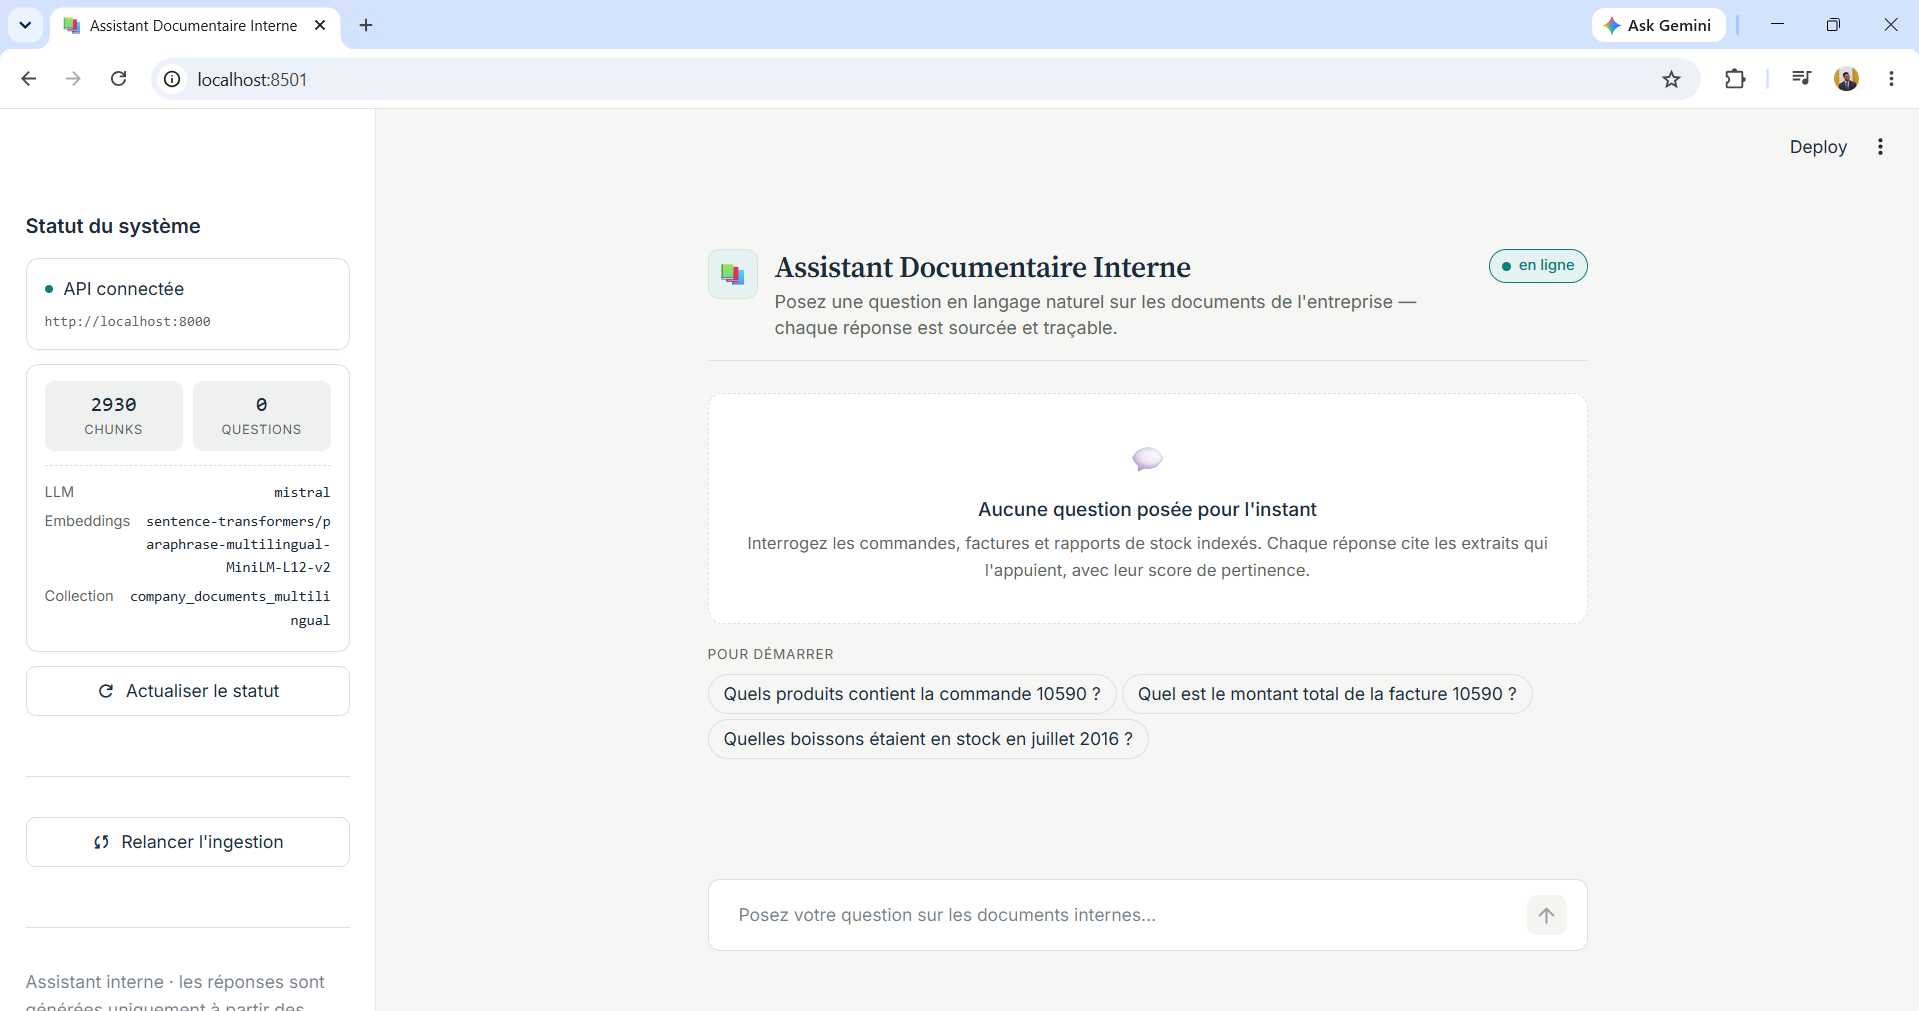
\includegraphics[width=\textwidth]{ui-accueil.png}
\caption{Écran d'accueil de l'assistant. La barre latérale affiche l'état du
système ; la zone centrale propose des questions d'amorçage cohérentes avec le
corpus indexé.}
\label{fig:ui-accueil}
\end{figure}

\subsection{Réponse sourcée}

La figure~\ref{fig:ui-reponse} montre le système en fonctionnement sur une
question réelle. La réponse est structurée, chaque bon de commande étant restitué
avec son identifiant, sa date, le produit concerné, la quantité et le prix
unitaire. Elle se termine par la liste explicite des fichiers sources utilisés.

Au-dessus de la réponse figure une ligne de métadonnées de traçabilité : le
nombre d'extraits mobilisés, le meilleur score de pertinence obtenu et le temps
de génération. Un panneau dépliable « Provenance » donne accès au détail de
chaque extrait, avec son identifiant de segment et une barre indiquant
visuellement son score.

\begin{figure}[htbp]
\centering
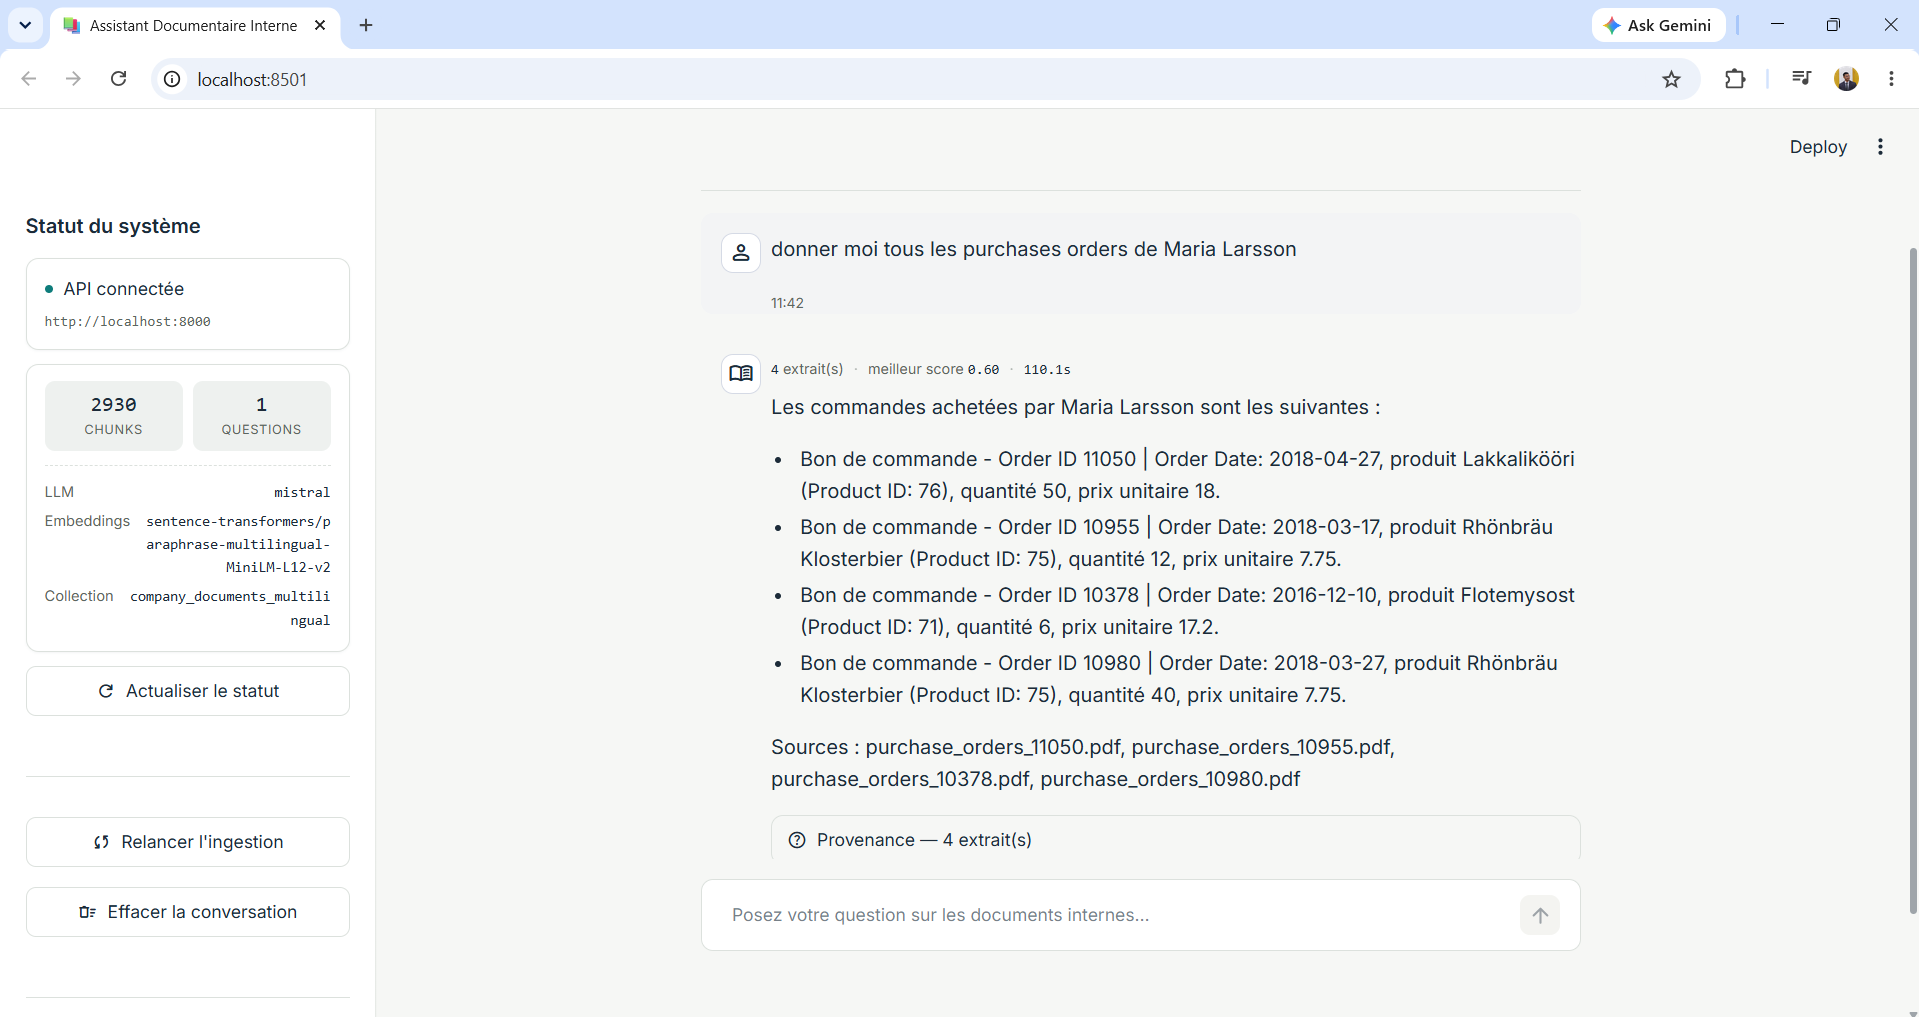
\includegraphics[width=\textwidth]{ui-reponse.png}
\caption{Réponse sourcée produite par le système. Les quatre bons de commande
sont restitués avec leurs détails, suivis de la liste des fichiers sources. La
ligne de métadonnées indique le nombre d'extraits, le meilleur score et le temps
de génération.}
\label{fig:ui-reponse}
\end{figure}

Cet affichage constitue la traduction concrète du critère de traçabilité fixé au
chapitre~\ref{ch:metier}. L'utilisateur n'a pas à croire le système : il peut
ouvrir les fichiers cités et vérifier. C'est ce qui distingue un assistant
exploitable en entreprise d'une démonstration technique.

\section{Conteneurisation avec Docker}

\subsection{Organisation}

Le déploiement repose sur trois services orchestrés par \texttt{docker compose},
décrits au tableau~\ref{tab:services}.

\begin{table}[htbp]
\centering
\caption{Services définis dans \texttt{docker-compose.yml}}
\label{tab:services}
\small
\begin{tabularx}{\textwidth}{@{}p{2.7cm}p{1.5cm}p{3.1cm}X@{}}
\toprule
\textbf{Service} & \textbf{Port} & \textbf{Image} & \textbf{Rôle} \\
\midrule
\texttt{rag-ollama} & 11434 & \texttt{ollama/ollama} &
Sert le modèle Mistral 7B ; volume persistant pour les poids \\
\texttt{rag-api} & 8000 & \texttt{Dockerfile.api} &
Moteur RAG et API REST ; monte \texttt{./data} pour accéder à l'index \\
\texttt{rag-streamlit} & 8501 & \texttt{Dockerfile.streamlit} &
Interface web ; ne connaît que l'URL de l'API \\
\bottomrule
\end{tabularx}
\end{table}

Deux volumes assurent la persistance : \texttt{ollama\_data} conserve les poids
du modèle, évitant un téléchargement de 4,4~Go à chaque redémarrage, et
\texttt{./data} conserve l'index ChromaDB, évitant une ré-ingestion complète.

La configuration inter-services s'effectue par variables d'environnement, les
conteneurs se résolvant par leur nom de service sur le réseau Docker interne :

\begin{lstlisting}[style=plain,caption={Extrait de \texttt{docker-compose.yml}}]
  api:
    build: { context: ., dockerfile: Dockerfile.api }
    container_name: rag-api
    ports: ["8000:8000"]
    environment:
      - OLLAMA_BASE_URL=http://ollama:11434
      - CHROMA_PERSIST_DIR=/app/data/processed/chroma_db
    volumes: ["./data:/app/data"]
    depends_on: [ollama]
\end{lstlisting}

\subsection{Mise en service}

Le déploiement complet tient en deux commandes :

\begin{lstlisting}[style=bash,caption={Déploiement conteneurisé}]
docker compose up --build -d
docker exec -it rag-ollama ollama pull mistral
\end{lstlisting}

La seconde commande télécharge les poids du modèle dans le conteneur Ollama. Elle
n'est nécessaire qu'au premier démarrage, le volume persistant conservant
ensuite le modèle.

L'ingestion du corpus s'effectue alors par simple appel à l'API :

\begin{lstlisting}[style=bash,caption={Ingestion via l'API}]
curl -X POST http://localhost:8000/ingest \
     -H "Content-Type: application/json" \
     -d '{"reset": true}'
\end{lstlisting}

\section{Points de vigilance avant mise en production}

L'état actuel du déploiement est fonctionnel en environnement de développement,
mais plusieurs points doivent être traités avant toute exposition réelle. Ils
sont recensés au tableau~\ref{tab:vigilance} par ordre de criticité.

\begin{table}[htbp]
\centering
\caption{Points de vigilance identifiés}
\label{tab:vigilance}
\small
\begin{tabularx}{\textwidth}{@{}p{4.1cm}p{2.1cm}X@{}}
\toprule
\textbf{Point} & \textbf{Criticité} & \textbf{Action requise} \\
\midrule
Dépendances non figées &
\aremplir{Bloquant} &
Plusieurs modules importés par le code (\texttt{pypdf}, \texttt{python-docx},
\texttt{sentence-transformers}, \texttt{httpx}, \texttt{ragas},
\texttt{datasets}) ne figurent pas dans \texttt{requirements.txt}. La
construction des images Docker produit donc des conteneurs incomplets. Ce
fichier doit être complété et les versions figées \\
\addlinespace
Absence d'authentification & Élevée &
L'API et l'interface n'ont aucun contrôle d'accès. Ajouter une clé d'API ou
OAuth, et placer un \eng{reverse proxy} avec HTTPS devant l'interface \\
\addlinespace
Exposition des services internes & Élevée &
Restreindre l'accès réseau à Ollama et ChromaDB, qui ne doivent pas être
joignables publiquement \\
\addlinespace
Journalisation d'audit & Moyenne &
Tracer qui a posé quelle question et quelles sources ont été mobilisées, à des
fins de conformité \\
\addlinespace
Filtrage des documents sensibles & Moyenne &
Anonymiser ou exclure les documents à caractère personnel avant ingestion
(RGPD) \\
\addlinespace
Latence de génération & Moyenne &
Prévoir un GPU ou un modèle quantifié pour un usage quotidien
(\emph{cf.} chapitre~\ref{ch:evaluation}) \\
\bottomrule
\end{tabularx}
\end{table}

Le premier point mérite un commentaire. Il illustre un écueil classique du
développement : l'environnement local a été enrichi progressivement par
installations successives, sans que le fichier de dépendances soit tenu à jour.
Le code fonctionne donc parfaitement sur la machine de développement tout en
étant irreproductible ailleurs --- ce qui est précisément ce que la
conteneurisation est censée éliminer. La leçon est de valider systématiquement
une construction depuis un environnement vierge, et non depuis l'environnement de
travail.

\section{Versionnement}

Le code source est versionné avec Git. L'arborescence du projet sépare
explicitement les responsabilités, comme le montre le
listing~\ref{lst:arbo}.

\begin{lstlisting}[style=plain,caption={Organisation du dépôt},label={lst:arbo}]
rag-enterprise-assistant/
|-- src/
|   |-- config.py              # configuration centralisee (.env)
|   |-- ingestion/             # chargement, decoupage, indexation
|   |-- rag/                   # recherche, generation, pipeline
|   |-- evaluation/            # metriques RAGAS
|   |-- api/                   # backend FastAPI
|   +-- app/                   # interface Streamlit
|-- scripts/ingest_documents.py
|-- data/
|   |-- raw/                   # corpus source
|   |-- processed/             # index ChromaDB persiste
|   +-- eval/testset.csv       # jeu d'evaluation
|-- tests/
|-- docs/                      # architecture, guide de deploiement
|-- Dockerfile.api
|-- Dockerfile.streamlit
|-- docker-compose.yml
|-- Makefile
+-- requirements.txt
\end{lstlisting}

Un \texttt{Makefile} centralise les opérations courantes
(\texttt{make ingest}, \texttt{make api}, \texttt{make ui}, \texttt{make eval},
\texttt{make test}), ce qui réduit le risque d'erreur de manipulation et
documente de fait les commandes utiles du projet.

\section{Conclusion}

Ce chapitre a présenté le déploiement du système en trois services conteneurisés :
un serveur de modèle Ollama, une API REST FastAPI exposant quatre
\eng{endpoints}, et une interface conversationnelle Streamlit. Le découplage
strict entre l'interface et le moteur permet de substituer l'une sans toucher à
l'autre. Les captures présentées attestent du fonctionnement effectif de la
chaîne complète, de la question posée jusqu'à la réponse sourcée accompagnée de
ses extraits et de leurs scores. Les points de vigilance à traiter avant une
exposition réelle ont été recensés, le plus critique étant la complétion du
fichier de dépendances.


% ============================================================
%  Conclusion Générale
% ============================================================
\chapter*{Conclusion Générale}
\addcontentsline{toc}{chapter}{Conclusion Générale}
\markboth{Conclusion Générale}{}

Ce stage a été consacré à la conception, à la réalisation et au déploiement d'un
système RAG (\eng{Retrieval-Augmented Generation}) permettant d'interroger en
langage naturel un corpus de documents d'entreprise, avec des réponses sourcées
et vérifiables. Le travail a été conduit selon la méthodologie CRISP-DM, dont
chaque phase a été traitée successivement : compréhension du besoin métier,
exploration et préparation d'un corpus de 2\,676 documents, construction de la
chaîne de traitement, évaluation de sa fiabilité et déploiement conteneurisé.

\section*{Bilan du travail réalisé}

Sur le plan fonctionnel, la chaîne complète est opérationnelle. Le pipeline
d'ingestion traite les cinq formats documentaires courants, extrait le texte,
l'enrichit de métadonnées de traçabilité et le découpe en segments : les 2\,676
fichiers du corpus ont été intégralement traités, sans aucun échec d'extraction,
produisant 2\,929 segments vectorisés et persistés dans ChromaDB. La recherche
sémantique s'exécute en 182~millisecondes en moyenne. La génération est assurée
localement par Mistral 7B, contraint par une invite qui lui interdit de sortir du
contexte fourni. L'ensemble est exposé par une API REST à quatre
\eng{endpoints} et une interface conversationnelle, déployés en trois conteneurs
Docker.

La contrainte structurante du projet a été respectée sans concession :
\textbf{aucune donnée ne quitte l'infrastructure}. Vectorisation, indexation,
recherche, génération et même l'évaluation par modèle juge s'exécutent
localement, sans clé d'API ni coût récurrent. Cette propriété, qui aurait pu
paraître une contrainte appauvrissante, s'est révélée le principal argument de
l'architecture retenue face aux solutions du marché.

Sur le plan de la traçabilité, l'objectif est atteint. Chaque réponse expose les
fichiers sources mobilisés, l'identifiant précis de chaque segment et son score
de pertinence. L'utilisateur peut vérifier ce que le système avance plutôt que de
devoir lui faire confiance --- ce qui constitue, en contexte professionnel, la
condition d'adoption d'un outil de ce type.

\section*{Principal apport de la démarche d'évaluation}

Le résultat le plus instructif du stage n'est pas la mise en service du système,
mais ce que sa mesure a révélé. À l'usage, l'assistant produisait des réponses
d'apparence satisfaisante. L'évaluation quantitative de la composante de
recherche a pourtant montré que les scores de pertinence étaient anormalement
faibles sur des questions posées en français, et que le système s'appuyait
fréquemment sur des documents inadaptés.

Une expérience contrôlée a permis d'en identifier et d'en quantifier la cause :
à contenu sémantique identique, la traduction d'une question en anglais
\textbf{triple le score de pertinence} (0,461 contre 0,153 en moyenne). Le modèle
\texttt{all-MiniLM-L6-v2}, entraîné essentiellement sur de l'anglais, projette
mal les questions françaises dans l'espace sémantique de documents anglophones.

Ce constat porte un enseignement méthodologique qui dépasse le cas particulier :
\textbf{un système RAG peut paraître fonctionner tout en s'appuyant sur les
mauvais documents}. Une réponse fluide, bien structurée et accompagnée de sources
n'est pas pour autant une réponse correcte. Seule la mesure permet de distinguer
les deux, et c'est ce qui justifie la place centrale que CRISP-DM accorde à la
phase d'évaluation avant tout déploiement.

\section*{Limites du travail}

Trois limites doivent être clairement énoncées.

La \textbf{campagne d'évaluation RAGAS n'a pas été menée à son terme}. Le module
de mesure est développé et configuré pour fonctionner avec un modèle juge local,
mais son exécution requiert la constitution préalable d'un jeu de questions
annotées de réponses de référence rédigées manuellement. Les quatre métriques ---
\eng{faithfulness}, \eng{answer relevancy}, \eng{context precision} et
\eng{context recall} --- restent donc à mesurer. Le choix a été fait de laisser
ces valeurs explicitement vacantes dans le présent rapport plutôt que de les
estimer.

Le \textbf{corpus est exclusivement transactionnel}. Les 2\,676 documents sont
des factures, bons de commande, commandes et états de stock, c'est-à-dire des
enregistrements structurés. Ils permettent de valider techniquement le pipeline,
mais ils sous-exploitent l'intérêt propre d'une architecture RAG, qui donne son
plein rendement sur des documents rédigés où l'information est diffuse. Sur des
enregistrements structurés, une requête SQL serait plus exacte et plus rapide.
Cette composition explique par ailleurs le caractère quasi inopérant du paramètre
de découpage, la longueur moyenne d'un document (498 caractères) étant très
inférieure à la taille de segment configurée (1\,000 caractères).

La \textbf{latence de génération est excessive} pour un usage quotidien : environ
110 secondes par réponse. L'inférence d'un modèle de 7 milliards de paramètres
sur CPU représente plus de 99~\% du temps de réponse total, la recherche
vectorielle étant quant à elle négligeable.

\section*{Perspectives}

Les travaux futurs se hiérarchisent naturellement à partir des mesures obtenues.

\paragraph{Adopter un modèle d'\eng{embeddings} multilingue.}
C'est l'action de rang le plus élevé, car la plus étayée expérimentalement. Le
remplacement de \texttt{all-MiniLM-L6-v2} par
\texttt{paraphrase-multilingual-MiniLM-L12-v2}, entraîné sur plus de cinquante
langues, devrait résoudre l'asymétrie linguistique documentée au
chapitre~\ref{ch:evaluation}. L'opération impose une ré-indexation complète du
corpus.

\paragraph{Conduire la campagne RAGAS.}
Une fois le modèle multilingue en place, la constitution d'un jeu de vingt
questions annotées permettra d'établir une mesure de référence des quatre
métriques, et surtout de comparer objectivement les configurations successives
plutôt que de se fier à une impression d'usage.

\paragraph{Mettre en place une recherche hybride.}
La combinaison d'une composante lexicale exacte (BM25) et de la composante
vectorielle, avec fusion des classements, lèverait la limite documentée sur la
recherche par identifiant exact --- besoin fréquent sur un corpus transactionnel
où l'utilisateur connaît souvent le numéro de la pièce qu'il cherche.

\paragraph{Ajouter un ré-ordonnancement.}
L'insertion d'un \eng{cross-encoder} après la recherche vectorielle, chargé de
réévaluer finement la pertinence des extraits candidats, améliorerait la
\eng{context precision} et permettrait d'établir enfin un seuil de rejet fiable.

\paragraph{Enrichir le corpus de documents rédigés.}
L'ajout de procédures, manuels et notes d'organisation permettrait d'exercer le
système sur le type de questions pour lequel une architecture RAG est réellement
supérieure aux alternatives, et redonnerait au réglage du découpage son rôle de
levier d'optimisation.

\paragraph{Réduire la latence.}
Le passage sur GPU, l'emploi d'un modèle plus fortement quantifié ou plus petit,
et la diffusion progressive de la réponse constituent trois leviers cumulables.

\vspace{0.5cm}

En définitive, ce stage a permis de mener un projet de science des données de la
formulation du besoin jusqu'à un système déployé et mesurable, en abordant
l'ensemble de la chaîne : ingénierie documentaire, recherche sémantique,
ingénierie d'invite, évaluation de systèmes génératifs et déploiement
conteneurisé. Au-delà des compétences techniques acquises, l'apport principal
réside dans une conviction méthodologique : dans un système fondé sur un modèle
génératif, la qualité perçue est un indicateur trompeur, et l'instrumentation de
la mesure n'est pas une étape finale de validation mais la condition même du
progrès.


% ============================================================
%  Bibliographie / Nétographie
% ============================================================
\chapter*{Bibliographie et Nétographie}
\addcontentsline{toc}{chapter}{Bibliographie et Nétographie}
\markboth{Bibliographie et Nétographie}{}

\section*{Articles scientifiques}

\begin{enumerate}[label={[\arabic*]},leftmargin=2.2em]

\item P.~Lewis \emph{et al.}, « Retrieval-Augmented Generation for
Knowledge-Intensive NLP Tasks », \emph{Advances in Neural Information Processing
Systems (NeurIPS)}, 2020. \\
\url{https://arxiv.org/abs/2005.11401}

\item N.~Reimers et I.~Gurevych, « Sentence-BERT: Sentence Embeddings using
Siamese BERT-Networks », \emph{Proceedings of EMNLP-IJCNLP}, 2019. \\
\url{https://arxiv.org/abs/1908.10084}

\item N.~Reimers et I.~Gurevych, « Making Monolingual Sentence Embeddings
Multilingual using Knowledge Distillation », \emph{Proceedings of EMNLP}, 2020. \\
\url{https://arxiv.org/abs/2004.09813}

\item S.~Es, J.~James, L.~Espinosa-Anke et S.~Schockaert, « RAGAS: Automated
Evaluation of Retrieval Augmented Generation », \emph{Proceedings of EACL
(System Demonstrations)}, 2024. \\
\url{https://arxiv.org/abs/2309.15217}

\item A.~Q.~Jiang \emph{et al.}, « Mistral 7B », \emph{arXiv preprint}, 2023. \\
\url{https://arxiv.org/abs/2310.06825}

\item Y.~A.~Malkov et D.~A.~Yashunin, « Efficient and Robust Approximate Nearest
Neighbor Search Using Hierarchical Navigable Small World Graphs », \emph{IEEE
Transactions on Pattern Analysis and Machine Intelligence}, vol.~42, n\textsuperscript{o}~4,
2020. \\
\url{https://arxiv.org/abs/1603.09320}

\item V.~Karpukhin \emph{et al.}, « Dense Passage Retrieval for Open-Domain
Question Answering », \emph{Proceedings of EMNLP}, 2020. \\
\url{https://arxiv.org/abs/2004.04906}

\item L.~Huang \emph{et al.}, « A Survey on Hallucination in Large Language
Models: Principles, Taxonomy, Challenges, and Open Questions », \emph{ACM
Transactions on Information Systems}, 2024. \\
\url{https://arxiv.org/abs/2311.05232}

\item S.~E.~Robertson et H.~Zaragoza, « The Probabilistic Relevance Framework:
BM25 and Beyond », \emph{Foundations and Trends in Information Retrieval},
vol.~3, n\textsuperscript{o}~4, 2009.

\item R.~Wirth et J.~Hipp, « CRISP-DM: Towards a Standard Process Model for Data
Mining », \emph{Proceedings of the 4th International Conference on the Practical
Applications of Knowledge Discovery and Data Mining}, 2000.

\end{enumerate}

\section*{Documentation technique}

\begin{enumerate}[label={[\arabic*]},leftmargin=2.2em,start=11]

\item \textbf{LangChain} --- Documentation officielle du \eng{framework}
d'orchestration. \\
\url{https://python.langchain.com/docs/}

\item \textbf{ChromaDB} --- Documentation de la base de données vectorielle. \\
\url{https://docs.trychroma.com/}

\item \textbf{Ollama} --- Exécution locale de modèles de langue. \\
\url{https://ollama.com/}

\item \textbf{Sentence-Transformers} --- Bibliothèque de modèles
d'\eng{embeddings} de phrases. \\
\url{https://www.sbert.net/}

\item \textbf{RAGAS} --- \eng{Framework} d'évaluation de systèmes RAG. \\
\url{https://docs.ragas.io/}

\item \textbf{FastAPI} --- \eng{Framework} web asynchrone pour Python. \\
\url{https://fastapi.tiangolo.com/}

\item \textbf{Streamlit} --- Création d'applications web en Python. \\
\url{https://docs.streamlit.io/}

\item \textbf{Docker Compose} --- Orchestration de conteneurs multi-services. \\
\url{https://docs.docker.com/compose/}

\item \textbf{pypdf} --- Extraction de texte de fichiers PDF. \\
\url{https://pypdf.readthedocs.io/}

\item \textbf{Pydantic} --- Validation de données et gestion de configuration. \\
\url{https://docs.pydantic.dev/}

\end{enumerate}

\section*{Ressources et jeux de données}

\begin{enumerate}[label={[\arabic*]},leftmargin=2.2em,start=21]

\item \textbf{Company Documents Dataset} --- Corpus de documents d'entreprise
utilisé dans ce projet, Kaggle. \\
\url{https://www.kaggle.com/datasets/ayoubcherguelaine/company-documents-dataset}

\item \textbf{MTEB} (\eng{Massive Text Embedding Benchmark}) --- Classement
comparatif des modèles d'\eng{embeddings}, \eng{Hugging Face}. \\
\url{https://huggingface.co/spaces/mteb/leaderboard}

\item \textbf{all-MiniLM-L6-v2} --- Fiche du modèle d'\eng{embeddings} employé. \\
\url{https://huggingface.co/sentence-transformers/all-MiniLM-L6-v2}

\item \textbf{paraphrase-multilingual-MiniLM-L12-v2} --- Fiche du modèle
multilingue préconisé en perspective. \\
\url{https://huggingface.co/sentence-transformers/paraphrase-multilingual-MiniLM-L12-v2}

\end{enumerate}


\end{document}
